\documentclass[12pt,a4paper,twoside]{ctexrep}
\usepackage{Alegreya}
\usepackage{AlegreyaSans}
\usepackage{DejaVuSansMono}
\usepackage{csquotes}
\usepackage{amsmath}             % Split equations
\usepackage{mathpazo}
\usepackage{fontspec}
\usepackage{fancyhdr}
\usepackage[explicit]{titlesec}
\usepackage{graphicx}
\usepackage[table]{xcolor}
\usepackage{pbox}
\usepackage{tikz}
\usepackage{listings}            % Code syntax highlighting
\usepackage{ctable}
\usepackage{multirow}
\usepackage{dcolumn}             % Align columns by decimal position
\usepackage{float}               % Place figure or table HERE
\usepackage[hang,small]{caption} % Modify caption labels margin=20pt, tableposition=top, textfont=it
\usepackage{pdflscape}
\usepackage{eso-pic}             % Cover image
\usepackage{url}                 % Clickable URLs
\usepackage[bookmarks]{hyperref} % PDF with links. Goes AFTER all packages
\usepackage[all]{hypcap}         % Because the caption is set below the fig., so the fig. is not visible if a link jumps to a fig. Goes AFTER hyperref.
\usepackage{verbatim}
% **************************************************
% Fonts
% **************************************************
\defaultfontfeatures{Ligatures=TeX}
\setmainfont[Numbers=Lining]{Alegreya}
\setsansfont[Numbers=Lining]{Alegreya Sans}
\setmonofont{DejaVuSansMono}
\setmathrm{Alegreya}
\setmathsf{Alegreya Sans}
\setboldmathrm[BoldFont={Alegreya Bold}]{Alegreya}
% http://tex.stackexchange.com/questions/62603/how-to-choose-a-specific-weight-from-a-font-family-using-fontspec-and-xelatex
% **************************************************
% Colors
% **************************************************
\definecolor{blue}{RGB}{34,128,188}	% 0.13 0.50 0.73 
\definecolor{lightblue}{RGB}{199,234,253}
\definecolor{lightgray}{RGB}{230,230,230}
\definecolor{yellow}{HTML}{F3C50F}
\definecolor{green} {HTML}{9ACD32}
\definecolor{violet}{HTML}{990055}
% **************************************************
% Lengths
% **************************************************
\setlength{\parskip}{.5cm}
\setlength{\oddsidemargin}{17.3571pt}
\setlength{\evensidemargin}{17.3571pt}
\setlength{\marginparwidth}{35.0pt}
% **************************************************
% Captions
% **************************************************
\DeclareCaptionFont{sf}{\AlegreyaSansLight}
\DeclareCaptionFont{bf}{\AlegreyaSansMedium}
\captionsetup{width=0.8\textwidth}
\captionsetup{labelfont=bf,textfont=sf}
% **************************************************
% PDF output
% **************************************************
\hypersetup{
% --- Configuration options ---------------------------------------------------------------------------------------------------------------------
	breaklinks  = true,     % allow links to break over lines by making links over multiple lines into PDF links to the same target. 
% --- Extension options -------------------------------------------------------------------------------------------------------------------------
	linktoc     = page,     % section, slide, page, none, or all be link on TOC/LOF/LOT. Also linktocpage = true.
	colorlinks  = true,     % false: boxed links; true: colored links (boxed links are not printed). Only named colors work.
	linkcolor   = red,      % color of internal links
	urlcolor    = blue,     % color of external links
	citecolor   = blue,     % color of links to bibliography
% --- PDF-specific display options --------------------------------------------------------------------------------------------------------------
	linkbordercolor={1 0 0},            % The color of the box around normal links 	
	urlbordercolor ={0.13 0.50 0.73},   % The color of the box around links to URLs 
	citebordercolor={0.13 0.50 0.73},   % The color of the box around citations 
% --- PDF display and information options -------------------------------------------------------------------------------------------------------
	pdftitle     = {七堂物理概论课},                   % title
	pdfsubject   = {Physics},   % subject of the document
	pdfauthor={Carlo Rovelli[著];2017超越学科的认知基础课程全体同学[译]}
	pdfstartview = {FitV},                               % fits the height of the page to the window
} % ---------------------------------------------------------------------------------------------------------------------------------------------
% **************************************************
% Header and Footer
% **************************************************
\pagestyle{fancy}
% --- Nothing in the headers ---------------------------------------------------------------------------------------------------------------------
	\fancyhead{} \renewcommand{\headrulewidth}{0pt}
% --- Chapter in left page -----------------------------------------------------------------------------------------------------------------------
	\renewcommand{\chaptermark}[1]{%
		\markboth{%
			\color{gray!80!white}\footnotesize%
			{\AlegreyaSansBlack\textbf{\chaptername\ \thechapter}}%
			\quad%
			{\AlegreyaSansLight#1}%
		}{}%
	}

% --- Section in right page ---------------------------------------------------------------------------------------------------------------------
	\renewcommand{\sectionmark}[1]{%
		\markright{%
			\color{gray!80!white}\footnotesize%
			{\AlegreyaSansBlack\textbf{\thesection}}%
			\quad%
			{\AlegreyaSans\textit{#1}}%
		}%
	}%
\fancypagestyle{plain}{%
	\fancyhf{}
	\fancyfootoffset[OR]{1.85cm}
	\fancyfoot[OR]{%
		{\ }\AlegreyaSans%
		{\color{lightgray}\rule[-95pt]{1.25pt}{100pt}}%
		\hspace*{10pt}\begin{minipage}[b]{1.5cm}%
			\color{gray!80!white}\normalsize\textbf{\thepage}%
		\end{minipage}%
	}
	\fancyfootoffset[EL]{1.85cm}
	\fancyfoot[EL]{%
		\AlegreyaSans%
		\begin{minipage}[b]{1.5cm}%
			\raggedleft\color{gray!80!white}\normalsize\textbf{\thepage}%
		\end{minipage}%
		\hspace*{10pt}{\color{lightgray}\rule[-95pt]{1.25pt}{100pt}}%
	}
	\renewcommand{\headrulewidth}{0pt}
	\renewcommand{\footrulewidth}{0pt}
}
%
\fancypagestyle{maincontentstyle}{%
	\pagestyle{plain}
	\fancyhf{}
	\fancyfootoffset[OR]{1.85cm}
	\fancyfoot[OR]{%
		{\ }\AlegreyaSans\footnotesize%
		\rightmark%
		\hspace*{0.75cm}{\color{lightgray}\rule[-95pt]{1.25pt}{100pt}}%
		\hspace*{10pt}\begin{minipage}[b]{1.5cm}%
			\color{gray!80!white}\normalsize\textbf{\thepage}%
		\end{minipage}%
	}
	\fancyfootoffset[EL]{1.85cm}
	\fancyfoot[EL]{%
		\AlegreyaSans\footnotesize%
		\begin{minipage}[b]{1.5cm}%
			\raggedleft\color{gray!80!white}\normalsize\textbf{\thepage}%
		\end{minipage}%
		\footnotesize%
		\hspace*{10pt}{\color{lightgray}\rule[-95pt]{1.25pt}{100pt}}%
		\hspace*{0.75cm}\leftmark%
	}
}

% **************************************************
% User commands
% **************************************************
\providecommand{\e}[1]{\ensuremath{\times 10^{#1}}}
\newcommand{\bfi}{\begin{figure}}
\newcommand{\efi}{\end{figure}}
\newcommand{\bt}{\begin{tabular}}
\newcommand{\et}{\end{tabular}}
\newcommand{\bc}{\begin{center}}
\newcommand{\ec}{\end{center}}
\newcommand{\be}{\begin{equation}}
\newcommand{\ee}{\end{equation}}
\newcommand{\bi}{\begin{itemize}}
\newcommand{\ei}{\end{itemize}}
\newcommand{\ben}{\begin{enumerate}}
\newcommand{\een}{\end{enumerate}}
\newcommand{\pcen}{\relax\ifvmode\centering\fi\vspace*{.5ex}}
\newcommand{\code}[1]{\textbf{\texttt{\footnotesize #1}}}
\newcommand{\separator}{\bc\noindent\rule[2pt]{5mm}{0.1pt}$\sim \star \sim$ \rule[2pt]{5mm}{0.1pt}\ec} % Separator
\newcommand*\circled[1]{\tikz[baseline=(char.base)]{
	\node[shape=circle,draw,inner sep=2pt,fill=lightgray,lightgray!50!white] (char) {\color{gray}#1};}}
	\renewcommand{\labelenumi}{\protect\circled{\AlegreyaBlack\arabic{enumi}}}
	\renewcommand{\labelitemi}{\protect\circled{$\star$}}
	\renewcommand{\labelitemii}{\color{yellow}$\star$}
\newcommand\BackgroundPic{%
	\put(-126,0){
		\parbox[b][210mm]{297mm}{%
			\vfill
			\centering
			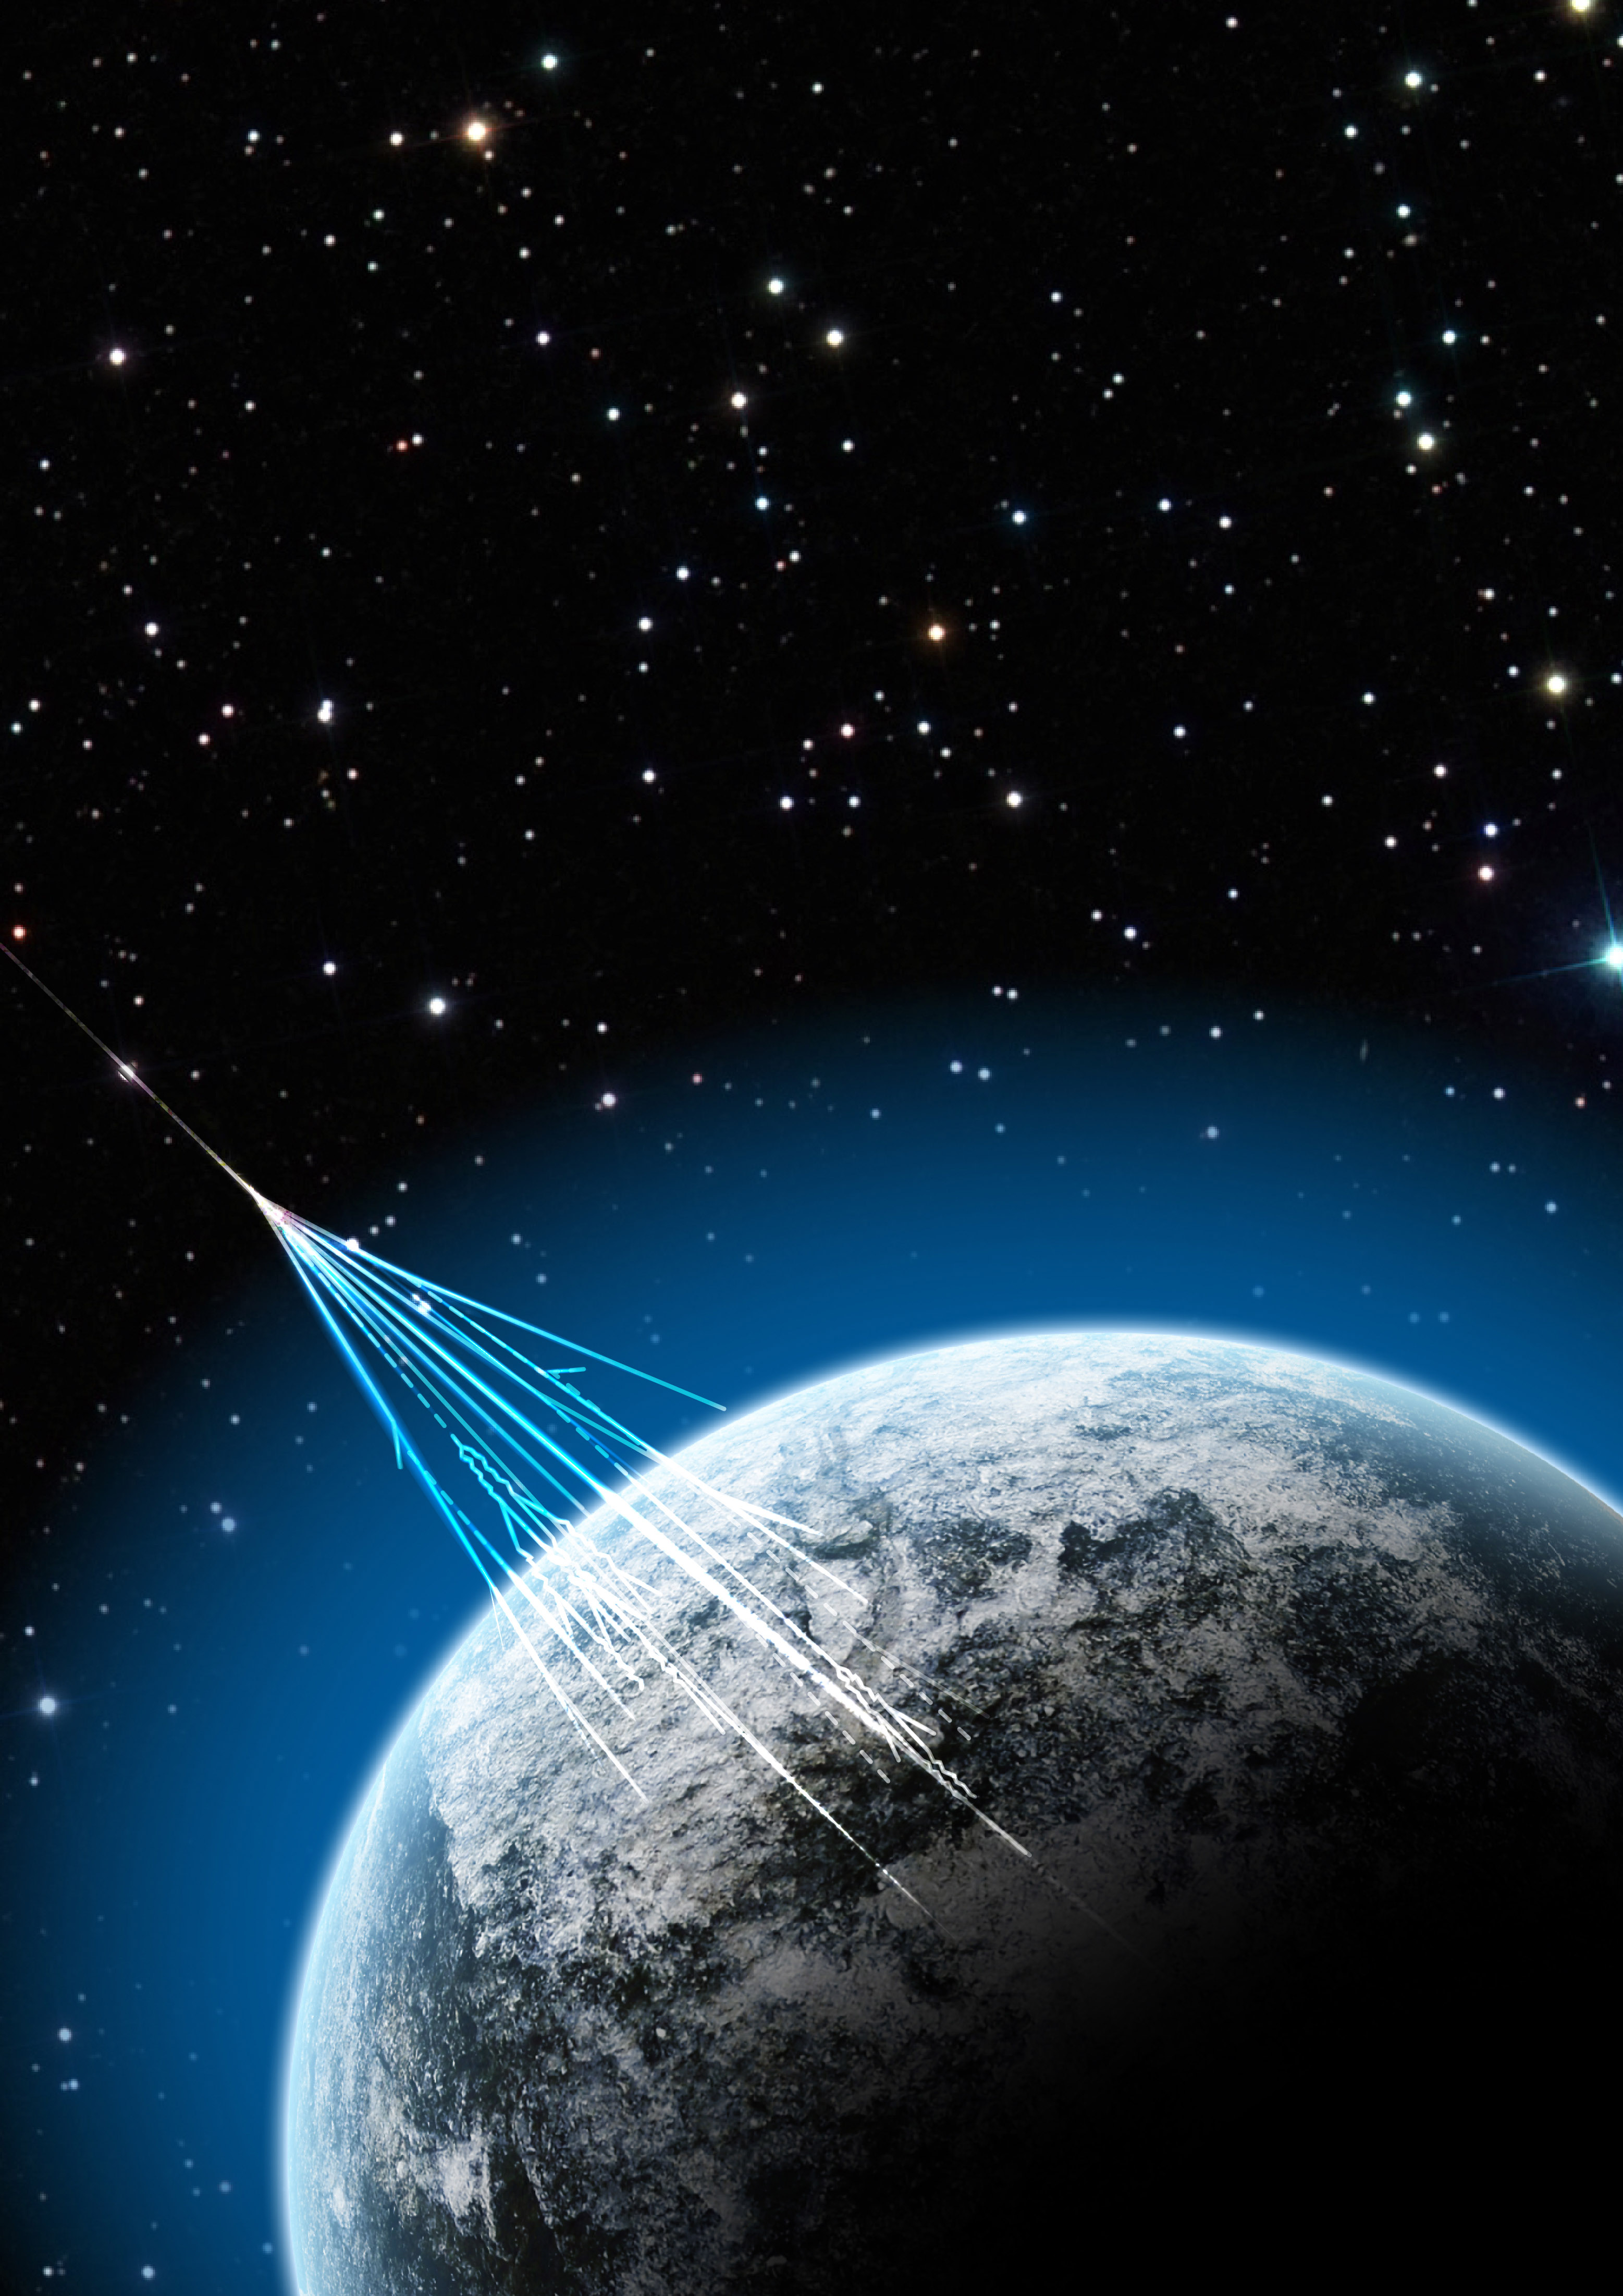
\includegraphics[width=210mm,keepaspectratio]{img/cover.jpg}%
			\vfill
		}%
	}%
}%
\newcommand{\graybox}[3]{%
	\bc\fcolorbox{lightgray}{lightgray!50!white}{%
		\parbox{#1\textwidth}{%
			\bc\parbox{#2\textwidth}{#3}\ec
		}%
	}\ec\par
}
% Fuzz
\hfuzz2pt % Don't bother to report over-full boxes if over-edge is < 2pt
% Listings
\lstset{
	language        = C++,
	breaklines      = true,
	tabsize         = 4,
	frame           = single,
	numbers         = left,
	numberstyle     = \color{gray}\sffamily,
    basicstyle      = \color{violet}\scriptsize\ttfamily,
	keywordstyle    = \color{green!90!black}\bfseries,
	identifierstyle = \color{black},
	commentstyle    = \color{gray}\itshape, % white comments
	stringstyle     = \color{blue},
	showstringspaces= false,
	rulecolor       = \color{lightgray},
	backgroundcolor = \color{lightgray!50!white}
}


\begin{document}

	% Cover and credits -----------------------------------------------------------
	\thispagestyle{empty}
	\pdfbookmark[0]{Cover}{cover}
		\AddToShipoutPicture*{\BackgroundPic}

	\begin{center}

		\vspace*{-2cm}
		\color{white}

		\hrule % --------------------------------------------------------------------------------------

		\Huge{\textsc {\textbf{\youyuan 七堂物理概论课}}}

		\large{\textsc {\textbf{Seven Brief Lessons on Physics}}}
		\vspace*{2ex}

		\hrule % --------------------------------------------------------------------------------------
		
		 
		\begin{large}
			\color{white}
			\textbf{
				\\
				\textit{
					Carlo Rovelli[著]\\
					2017超越学科的认知基础课程全体同学[译]
				}%
			}%

			\vfill

			October 2017
		\end{large}

		\vspace*{-3cm}

	\end{center}

	\newpage
	\thispagestyle{empty}
	\phantom{hola!}
		
	% Copyright and Credits	
	\null
	\vfill
	\bc
		\begin{minipage}{0.65\textwidth}
			{\sffamily
				\bc
					\textbf{\copyright 2017 \href{http://toyhouse.cc/wiki/index.php/Seven_Brief_Lessons_on_Physics}{\textbf{超越学科界限的认知基础}}}\\
					\textsc{Creative Commons}\\
					Attribution-NonCommercial 4.0 International\\
					\href{http://creativecommons.org/licenses/by-nc/4.0/legalcode}{(CC BY-NC 4.0)}\\[12pt]
					
\includegraphics{img/license.png}\\[12pt]
				\ec
	
				\small\textbf{Cover image:} Little is known about the ultra high-energy cosmic rays that regularly penetrate the atmosphere. Recent IceCube research rules out the leading theory that they come from Gamma Ray Bursts. (Courtesy: NSF/J. Yang).
			}
		\end{minipage}\vspace*{1ex}
		\small\href{http://www.interactions.org/cms/?pid=2100&image_no=DE0106}{\textbf{\url{http://www.interactions.org/cms/?pid=2100&image_no=DE0106}}}
	\ec

	\cleardoublepage

	% Table of contents -----------------------------------------------------------
	%    Title aligned right and in italics
	\titleformat{\chapter}[block]{\raggedleft\itshape}{}
		{0pt}{\parbox{\linewidth}{\raggedleft\vspace*{1em}\Huge#1}}
	\pdfbookmark[0]{Contents}{contents}
	\pagenumbering{roman}           % roman page numbering (invisible for empty page style)

	\pagestyle{plain}               % display just page numbers
	\tableofcontents
	\cleardoublepage

		\chapter*{序言}
	\indent

这本书是为那些对现代科学知之甚少的人们所写的。本书中的章节一起为读者提供了20世纪物理学最迷人的几个方面发生的革命,以及革命中提出的问题和迷的概况。科学不仅告诉我们怎样更好的了解世界,还启示我们这个世界的广阔以及无数未知事物的存在。

第一章主要讲爱因斯坦的相对论的一般理论,‘这些理论中最漂亮的一个’。第二章主要讲述量子力学,其中包含着现代物理学中最令人难以理解的部分。第三章主要讲述宇宙:我们所居住的宇宙的结构;第四章介绍基本的粒子。第五章介绍量子引力:这个理论正尝试着将20世纪的发现融合起来建立新的理论。第六章介绍黑洞存在的可能性以及黑洞的高温。本书的最后一章回归到我们自身,并且提问在这个物理学视角描述下的奇怪世界中我们看待自身存在的可能性。

这些章节是作者在意大利的一份周日报纸II Sole 24 Ore上发表的一系列文章的扩展。我想特别感谢Armando Massarenti,他认为应该允许科学方面的文章刊载在周日报纸的文化板块中,并且重视我们完整文化之中重要的一个方面——科学所扮演的角色。
	\noindent
	\cleardoublepage

	% Document body ---------------------------------------------------------------
	%	 Title over a yellow background
	\titleformat{\chapter}{\normalfont}{}
		{0pt}
		{\begin{tikzpicture}[remember picture,overlay]
			\node[yshift=-7cm] at (current page.north west)
				{\begin{tikzpicture}[remember picture, overlay]
					\draw[fill=yellow,yellow] (0,-1) rectangle
						(\paperwidth,7cm);
					\node[anchor=west,xshift=2\marginparwidth,yshift=2.5cm,rectangle]
						{\fontsize{380}{130}\color{white}\selectfont\AlegreyaBlack\thechapter};
					\node[anchor=west,xshift=2.5\marginparwidth,yshift=1cm,rectangle]
						{\parbox{\linewidth}{\raggedleft\vspace*{1em}\fontsize{40}{45}\selectfont\AlegreyaBlack#1}};
				 \end{tikzpicture}
				};
		 \end{tikzpicture}
		}
	\titlespacing*{\chapter}{0pt}{100pt}{0pt}

	\pagenumbering{arabic}          % arabic page numbering
	\setcounter{page}{1}            % set page counter
	\pagestyle{maincontentstyle}    % fancy header and footer
		\chapter{最美丽的理论}
\indent

	阿尔伯特·爱因斯坦在年轻的时候有一年都在漫无目的地游手好闲。不幸的是,如果你不“浪费”时间的话,你不会获得任何东西——这一点是青年人的父母常常会遗忘的。他那时在帕维亚。他去那里与家人会合,这时的他不得不中断了德国的学业,无法在那里度过充实的高中生活。那时正是二十世纪初,意大利正在工业革命的初级阶段。他的父亲是一名工程师,正在潘丹(paduan)平原建立第一台电力工厂。阿尔伯特那时正在阅读康德的著作,有时还会旁听帕维亚大学的课程:这只是为了开心,而不需要在那里登记或者需要为考试着想。就是在这样的情况下,严肃的科学家才诞生。

   在登记入学苏黎世联邦理工学院后,他沉浸于物理学的世界中。几年后,1905年,他在当时最为著名的科学杂志,the Annalender Physik上发表了三篇文章。这三篇文章每一篇都是诺贝尔奖级别的文章。第一篇文章揭示了原子的存在性。第二篇文章为量子力学奠定了最初的基础,我将在下一章详细阐述。第三篇文章提出了他关于相对论最初的理论(今天称之为狭义相对论),这一理论揭示了对于不同的人来说,时间并不是以相同的速度流逝的:如果其中一人以很快的速度移动,那么两个孪生子会发现他们年龄不同。

   爱因斯坦一夜之间成为了一位著名的物理学家并得到了许多高校的聘书。但是还是有一些事情使他烦躁:尽管这一理论产生了轰动效应,但它并没有与我们所知的引力发生联系,即物理下落的原因。当他为他的理论写一篇总结时,他意识到这一点,并开始思考由现代物理学之父牛顿所提出的引力公式是否需要修改,以使其与新的相对性观念相吻合。他埋头于这一问题中,他花了十年时间去解决这一问题。这十年时间充满了枯燥的学习,尝试,错误,混乱,错误的文章,新奇的想法和被误解的观点。

   最终,在1915年的11月,他呈递了一份彻底解决这一问题的文章:一个关于引力的新理论,他称之为广义相对论——这是他的杰作,被伟大的俄罗斯物理学家列夫·朗道称为“最美丽的理论”。

   有很多的杰作使我们十分感动:莫扎特的安魂曲;荷马的奥德赛;西斯廷教堂;李尔王。去完全欣赏它们的优美之处往往需要很长的学徒期,但是这种奖赏是纯粹的美丽——但是又不止于此,这一理论使我们有了一种崭新的审视世界的视角。爱因斯坦的宝石,广义相对论,是描述自然界秩序的杰作。

   我还记得我开始理解广义相对论的兴奋与激动。那是一个夏天,我正在卡拉布里亚的Condofuri的海滩上,沐浴在希腊地区地中海的阳光下,还有一年就要大学毕业。一个人只有在不被上学分心的时候,才能最佳地学习。我那时正在一本被老鼠咬破边缘的书的帮助下学习,这是因为在晚上我用这本书来堵住一个位于Umbrian山丘上的破旧房子的老鼠洞,从前我常常在这间房子里来逃避一些无聊的大学课程。我总是会从书中抬起头看远方波光粼粼的大海:我好像真正看见了爱因斯坦所想象的空间和时间的弯曲。这一切好像是魔法:好像是一个朋友在低声告诉我一个非凡的秘密,突然间揭开了现实的面纱,使之显露出一个更为简单也更为深刻的秩序。自从我们发现地球是圆的并且像一个陀螺一样不断自转,我们就已经发现现实并不是看上去那样:每次我们发现现实的一个新方面的知识,我们就会感受到一次深刻的情感体验。又一层面纱被我们撕掉了。

   但是在历史上超越我们的认知的一个接着一个的发现中,爱因斯坦或许是无可匹敌的。这是为什么呢?

   首先,一旦你理解了相对论,你就会发现它那优美的简洁性。我会总结这一观点。

   牛顿尽最大努力去解释物体要掉落和行星要公转的原因。他设想了一个使得所有物体聚集在一起的力,称之为引力。这个力在距离很远但是中间没有其它物体的物体之间发生作用的途径还是未知的——而且牛顿很谨慎地给出了一个假设。他想象物体在空间中移动,空间本身像一个非常大的空容器,大到将整个宇宙都囊括进入,在这个容器中的所有物体都各行其是,直到有力使它们的轨迹发生弯曲。这个牛顿发明的包括整个世界的容器——空间是由什么组成的,他自己也说不清楚。但是爱因斯坦出生后几年,两位伟大的英国物理学家迈克尔·法拉第和詹姆斯·麦克斯韦向牛顿的经典力学体系中添加了关键性的一部分:那就是电磁场。这个场是一个真实的实体,充斥空间,传播电磁波,可以像湖面一样振动,借此传递电磁力。由于爱因斯坦年轻的时候就被驱动他父亲所建立的发电厂中转子运动的电磁场所吸引,他不久后就理解了引力,像电场力一样,一定是被一个场所传播的:一个类比于电磁场的引力场一定是存在的。他的目标是理解引力场的工作规律,以及用数学方程式描述它。

   在那时他想到了一个非凡的想法,一个完全是天才的想法:引力场并不是充斥于空间的,引力场就是空间本身。这就是广义相对论的雏形。牛顿的空间,就是物体移动所有经过的空间,以及引力场是完全相同的一个事物。

   这是一个富有启迪的时刻。一个对于世界极为重要的简化:空间不再是和物质无关的事物,它也是一种组成这个世界的物质。它是一个可以弯曲的事物。我们并不是被装在一个僵硬的看不见的结构中:我们处于一个非常大的弹性蜗牛壳中。太阳使得它周围的空间弯曲,而地球也不是因为一种神秘的力才绕着太阳公转,它是因为它向太阳笔直前进,像一块大理石在漏斗表面滚动一样。在漏斗中央并不存在一个维持这一切的神秘的作用力;是被弯曲的空间导致了大理石的滚动。行星的绕日公转,以及物体的下落,都是因为空间被弯曲了。

   我们怎样才能描述空间的曲率呢?十九世纪最为杰出的数学家,有“数学王子”之称的卡尔·弗里德里希·高斯,已经提出了描述二维曲面,例如山丘表面,的数学方程式。之后,他让一个聪明的学生去将这一理论推广至三维乃至更多维空间中。回答这一问题的学生,伯纳德·黎曼,提出了一种对这一问题影响深远的基本原则,尽管看上去它完全是无用的。黎曼论述的结论是弯曲空间是被特定数学实体承载,这一数学实体我们今天称之为黎曼曲面,通常用R来标记。爱因斯坦提出了一个方程式,在这一方程式中R等价于物体的能量。这就是说空间在有物质存在的地方会发生弯曲。结论就是这样。(The equation fitsinto half a line, and there is nothing more)如果说这一等式解决了一半的问题,那么这里就没有其它的问题了。一个空间弯曲的观测结果变成了一个等式。

   但是,这一个方程式描述了整个宇宙。这一理论的丰富性在这里打开一连串幻觉似的的预言,这些预言像极了疯子的的胡言乱语,但是这些在之后都被证明是真的。

   首先,这一方程式描述了星体周围的空间是怎样弯曲的。因为曲率的存在,不仅仅行星绕着恒星公转,而且光线也不再沿着直线传播而是发生一定的偏转。在1919年,这一偏转被测量了出来,结果和理论符合的很好。但不仅仅空间会弯曲,时间也会弯曲。爱因斯坦预言在地球表面,相较于低处而言,在高处时间会流逝地更快。这也被实验所证实了。如果一个住在海平面高度的人和他住在山上的孪生兄弟相遇,他会发现他兄弟会比他稍稍老一点。而这才是刚刚开始。

   当一个大的星体烧尽了它所有的可燃烧的物质(氢)时,它就会坍塌。当剩余的部分不再能承载燃烧的热时,它就会由于自身的重量坍塌,直到它使得空间坍塌到产生一个真实的洞。这就是著名的黑洞。当我在大学学习这些时,它们仅仅被认为是这一复杂理论的可能预言。今天,他们被数以百计地观测出来,并被天文学家们仔细地研究。

   但这依旧不是全部内容。这个空间都可以膨胀或者收缩。而且,爱因斯坦的方程式揭示了空间不可能是静态的,它一定是在膨胀。在1930年,宇宙的膨胀被真正地观测出来。同样的一个方程预言这一膨胀应该是被一个年轻的非常小但非常热的宇宙爆发所引起的:现在我们称之为“大爆炸理论”。又一次,最初没有人相信这一理论,但是相关的证据一直积累到宇宙背景辐射——由于最初爆炸所产生扩散的微波——被直接观测到。爱因斯坦方程式所产生的预言又一次被证明是正确的。但是进一步,这一理论断言空间像大海的表面一样运动。这些引力波的影响在宇宙中的双星系统中被观测出来,又一次与这一理论的预言相吻合,甚至吻合到令人惊讶的一千亿分之一的数量级上。其它情况也是这样。

   简而言之,这一理论描述了一个多姿多彩并且令人惊奇的世界。在这里,宇宙爆炸,空间坍塌成为一个无底洞,时间在行星附近变得缓慢,无边无际的星际空间像大海表面一样波动……这所有的一切,都渐渐地在我那本被老鼠咬过的书中出现,但它们并不是一个精神错乱的白痴所讲的故事,也不是一个被卡拉比亚地区地中海的烈日和令人眩晕的大海所引发的幻觉。这一切都是现实。

   或者更好地说,现实的一小部分,只是现实所蒙上诸多面纱中的一小部分。这个现实似乎是由和构成我们梦境相同的事物所构成的,但是比我们朦胧的梦境更为真实。

   所有的这一切都是一个基本的直觉的结果:空间和引力场是同样的一个东西。尽管你们几乎一定不能去理解这一简单的方程式,但我还是要在这里写下它。或许任何读到这的人都能去欣赏它那完美的简洁性:

                                            $R_{ab}-1/2*Rg_{ab}=T_{ab}$

   就是这样。

   你或许,当然,为了掌握阅读和使用这一方程式需要去学习和理解黎曼的数学工具。这会耗费一些时间和精力。但是相对于欣赏贝多芬后期弦乐曲秘密的美丽,这都是次要的。在这两种情形下,奖赏都是纯粹的美丽,以及看待世界的一种崭新视角。

\noindent
\iffalse
	\graybox{.8}{.65}{
		\bc\textcolor{gray}{\Large{\sffamily Notation used in this document:}}\ec

		\textbf{Abbreviations:}

		EM: electro-magnetic,\\
		UV: ultra-violet,\\
		$\gamma$: gamma-rays,\\
		X: X-rays,\\
		$e^-$: electron,\\
		$\pi$: pion,\\
		$\mu$: muon,\\
		$\nu$: neutrino, etc.\vspace{2ex}

		\textbf{Units:}\\
		International System:\\
		eV: electron volts,\\
		J: Joules,\\
		C: Celsius,\\
		M: mega,\\
		G: giga, etc.\vspace{2ex}

		\textbf{Chemical symbols:}\\
		The elements of the periodic table.\vspace{2ex}

		\textbf{References:}\\
		There are internal (marked in \textcolor{red}{red}) and external (marked in \textcolor{blue}{blue}) references.\vspace{2ex}
	}
\fi

		\chapter{量子}
\indent

    二十世纪物理学的两大支柱——我在第一章所提到的广义相对论和现在我将要阐述的量子力学,不同到不能再不同了。这两个理论都告诉我们良好的自然结构比看上去更为细小。但是广义相对论是一个紧凑的佳作:作为由爱因斯坦自己思考到的成果,它是一个对于引力,空间和时间简单并且连贯的观点。而量子力学或“量子理论”,在另一方面,已经得到不相匹配的实验成功并且已经产生了改变我们每日生活的产品(例如,我正在使用的电脑)。但是在它诞生一个多世纪后,它还是十分神秘并且难以理解。

  据说量子力学是准确地在1900年诞生,几乎引导了一个世纪的很多思考。德国物理学家马克思.普朗克计算了黑体内的辐射场。为了计算,他用了一个巧妙的方法:他想象场的能量被分配在量子中,就是说能量被分为一块一块的。这一过程导致了和实验符合非常好的结果(因此,在一定程度上是正确的)但是却和当时所知的所有物理规律相违背。能量一直以来被认为是连续变化的,并且没有理由去把它处理成由小的结构单元组成。对普朗克本人来说,把能量处理成由有限的结构单元组成也是一种奇怪的计算方法,他自己也没有完全理解这种方法的有效性。再一次,是五年后爱因斯坦理解了能量单元是真实的。爱因斯坦认为光是由能量单元组成的——光单元。今天我们称它们为光子。他在他的文章的介绍中写道:我认为,如果我们假设光的能量是不连续分布在空间中,那么与黑体辐射,荧光,由紫外光激发的阴极射线以及其它与光产生与传播相关的物理现象都能够更好地被理解。与假设保持一致,点光源发射的光的能量在扩张的空间中是不连续分布的的,而且是由有限个位于空间中某个点的能量量子组成的,他们在移动中不会被拆分,只能作为整体产生或被吸收。

  这一段简洁而清晰的论断才是量子理论诞生的标志。注意到开始的“我认为”,使我想起了“我认为……”,就像达尔文介绍进化论时,或者法拉第第一次介绍关于磁场的革命性的理论时所说的。天才也是会犹豫的。

  爱因斯坦的工作最初被物理学界的同仁认为是一个杰出年轻物理学家无意义的幼稚之作。但是随后,因为同样的工作他被授予了诺贝尔奖。如果说普朗克是量子理论之父的话,那么爱因斯坦则是养育它的人。

  但是就像所有的后代一样,这一理论之后在爱因斯坦没有预料到的情况下自行发展。在二十世纪第二个和第三个十年,戴维·尼尔斯·玻尔领导了量子理论的发展。波尔理解了原子中电子的能量只能取固定的几个值,就像光的能量一样。重要的是,电子只能在能量一定的原子轨道之间跃迁,发射或吸收一个光子。这就是著名的量子跃迁。除此之外,在他位于哥本哈根的研究院内聚集了那个世纪最为杰出的青年物理学家,他们一起探索并且试图将原子世界一些令人困惑的现象澄清,最终建立一个连贯的理论。在1925年,这一理论的基本方程出现了,代替了全部的牛顿力学。

  很难想象比这更为杰出的成就了。一时间,所有事情都有意义了,你也可以计算所有的事情。例如:你是否还记得门捷列夫所发明的有这些周期和有这些特定性质的元素的结构?答案就是每个元素对应着量子力学主方程式的一个特解。化学由一个方程式产生。

  第一个依据那些令人眼花缭乱的假设写下这个方程的人,是德国的天才青年物理学家沃纳·海森堡。元素周期表,那上面列出了由氢到铀组成宇宙的所有可能的元素,因此被挂在很多教室的墙上。为什么就是这些元素被列举在这里以及为什么元素周期表

  海森堡认为电子并不总是存在的。它们只在有人或者仪器观察它们的时候,或者更准确地说,它们和其它事物发生相互作用的时候才存在。它们当与其它事物碰撞的时候,会在空间中以一定可计算的概率具象化。由一个轨道到另一个轨道量子跃迁是它们具象化的唯一方法:一个电子是一系列由一次相互作用到另一次相互作用的跃迁,电子并不位于任何准确的位置。它根本不在空间中。

  这就好像上帝并没有用一个加粗的线来设计现实,只是用点来描述它的轮廓。

  在量子力学中,不存在具有准确位置的物体,除了当它们飞快地和其它事物碰撞时。为了描述由一次相互作用到另一次相互作用的碰撞期间的物理过程,我们用一种不存在于真实物理空间,仅仅存在于抽象数学空间的抽象数学模型来刻画这一过程。但是更糟糕的事情发生了:这些相互作用的跃迁并不是以可预测的方式发生,而是很大程度上随机发生。我们不可能去预言电子将会在哪里重新出现,而只能去计算它会在这里或那里出现的概率。关于概率的问题深深困惑着那些认为所有事情都是由坚固、普遍并且不可动摇的物理学规律控制的物理学家们。   

   这听上去荒唐吗?这对爱因斯坦也十分荒唐。一方面,他提名海森堡获诺贝尔奖,因为意识到他理解了一些关于这世界基础的规律;另一方面,他不放过任何机会去抱怨这理论毫无意义。

   哥本哈根学派的年轻学者们十分沮丧:爱因斯坦怎么像这样来想?他们的精神领袖,那个曾经有勇气去思考不能思考的事物的大师,现在退缩了,畏惧这他自己所引发的到未知领域的跳跃。那个认为时间并不是永恒不变的和空间是卷曲的爱因斯坦现在却认为世界并不可能这样奇异。

  玻尔耐心地把这些新理论解释给爱因斯坦。爱因斯坦否认了这一理论。他设计了思想实验去证明这一新理论是自相矛盾的:“想象一个充满光的盒子,从这里我们允许单个的光子消失一瞬间……”之后就是他最著名的例子之一,“光盒(box of light)实验。最终波尔总能找到驳斥这些否认的答案。他们之间的对话以讲座,书信以及论文等等方式持续了很多年。在交换观点的过程中,这两位伟人都需要重新思考以调整他们的光点。爱因斯坦不得不承认新理论中不存在矛盾之处。玻尔不得不承认事情并不是像他一开始想的那样简单与清晰。爱因斯坦不想在总是存在一个不依赖于相互作用而存在的客观真实这一观点上让步。同样地,玻尔也不想在建构现实的新理论的可信性上让步。最终,爱因斯坦承认量子论是一个理解世界方面巨大的进步,但仍认为事物不应该像假设一样奇怪——这理论的背后一定存在一个更为深刻和理性的解释。

  一个世纪以后,我们现在面临着相同的问题。量子力学的方程及其解被物理学家,工程学家,化学家和生命科学家广泛地应用在不同的领域。它们在所有当代技术的领域都十分有用。但它们还是十分神秘。因为它们并没有描述物理系统内究竟发生了什么,只是刻画了一个物理系统是如何影响另一个物理系统的过程。

  这意味着什么?一个系统重要的真实性是不可描述的吗?这是否意味着我们只是缺少一部分谜题?或者这是否意味着,至少对我来说,我们必须接受现实仅仅是相互作用?我们在现实领域的知识总量在不断增加,这使得我们可以做一些我们过去甚至难以想象的事情。但是这增加又提出了新的问题,新的神秘。那些在实验室使用这些理论的人继续探索不管这些问题,但是在近些年数量急剧增加的文章和会议中,物理学家和哲学家继续去研究这些问题。在它诞生一个世纪以后,什么是量子理论?是一个对于自然真实性非常深刻的尝试?还是一个巧合与事实相符的大错?或是一个不完全谜题的一部分?亦或是一个深刻的关于世界结构的但我们目前还无法理解的理论的线索?

  爱因斯坦去世后,他最伟大的对手玻尔向他致以崇敬欣赏的悼词。当几年后玻尔去世时,有人拿出了他研究过程中的一块黑板的照片。在黑板上有一幅画。画所描述的是爱因斯坦思想实验中的“充满光的箱”。到最后,还是渴望去挑战自己以获得更多的认识与理解。到最后,还是对于事物本质的怀疑。

\noindent

		\chapter{宇宙的结构}
\indent

   在20世纪前半页, 爱因斯坦(Einstein)描述了时间与空间的原理, 与此同时, 尼尔斯·波尔(Niels Bohr)和他年轻的学徒醉心于描述物质的奇异的量子现象的方程. 在这个世纪的下半页, 物理学家在这两个理论基础之上, 把这两个全新的理论应用到描述自然现象的各个领域: 从宇宙的宏观结构到基本粒子的微观结构. 我将在这一章讲述前一个, 在下一张讲述后一个。

   这章主要由简单的草图组成. 这样的原因是在实验, 测量, 数学以及严密的推理之前, 科学最首要的是关于图像. 科学从图像开始. 科学思维是由从同以往不同的角度"看待"事物的能力培养出的. 我想在这里提供一个在不同看法间旅程的简要的, 适度的轮廓.
		
	\bc
	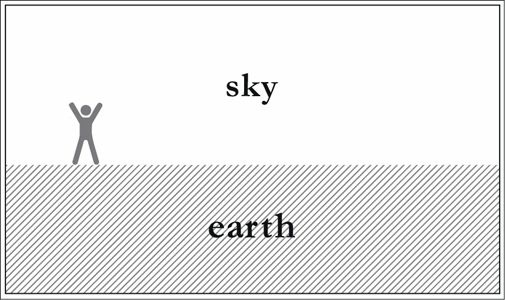
\includegraphics[width=.9\textwidth]{img/31.jpg}\\[12pt]
	\ec

   上面这张图代表了宇宙在数千年之间是如何被理解的: 土地在下面,天空在上面. 阿那克西曼德(Anaximander)在26个世纪之前完成了第一次伟大的科学革命, 他把上面的宇宙的图景换成了下面的样子,那时他正在试图弄清楚太阳, 月亮和星星是如何绕着我们旋转的.

	\bc
	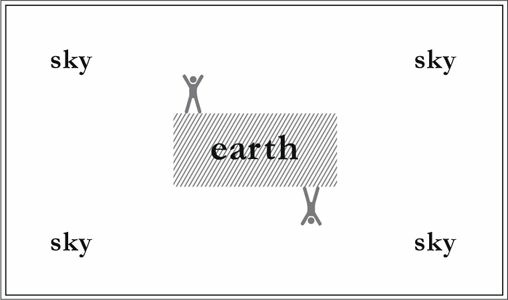
\includegraphics[width=.9\textwidth]{img/32.jpg}\\[12pt]
	\ec

   现在天空环绕在地球的四周, 而不仅仅是它的上方, 地球是悬挂在太空中的巨石, 没有落下. 很快有人(也许是帕门尼斯(Parmenides),也许毕达哥拉斯(Pythagoras))意识到, 球形是这个悬空的地球的最合理的形状, 因为其所有方向都是相同的, 亚里士多德(Aristotle)设计了令人信服的科学论证, 以证实地球和环绕地球四周的各种天体在其中运行的天空球形本质. 这是最后得到的宇宙的图像.

	\bc
	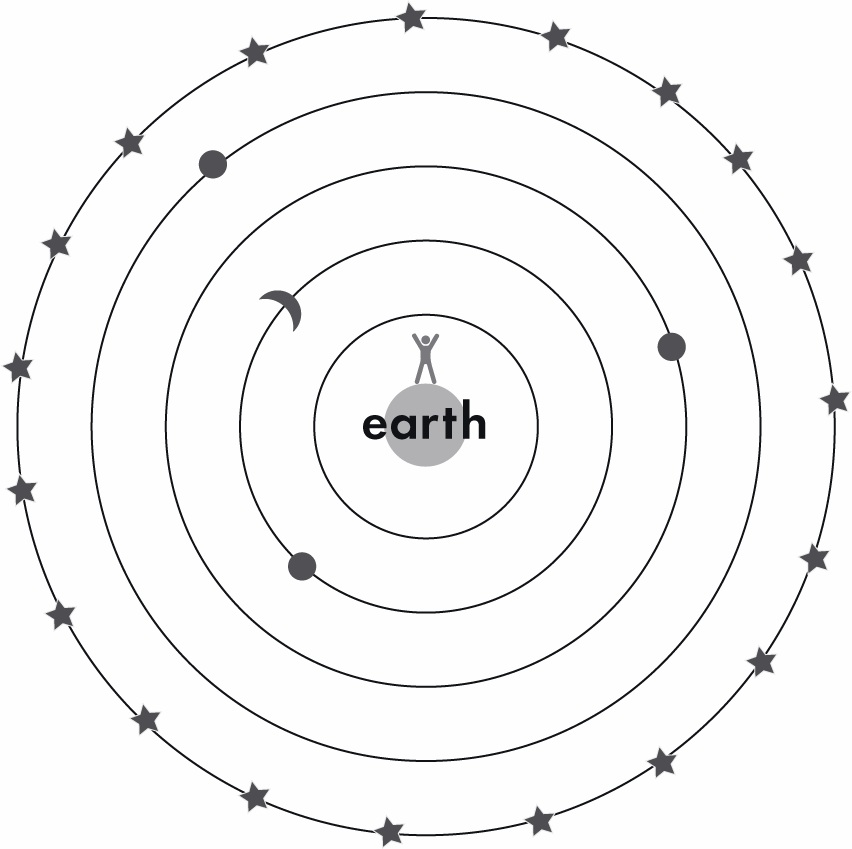
\includegraphics[width=.9\textwidth]{img/33.jpg}\\[12pt]
	\ec

   这个宇宙, 如亚里士多德(Aristotle)在他的作品"论天"中所描述的那样, 是世界的图像, 直到中世纪的结束, 它仍然是地中海文明的特征. 这是丹特(Dante)和莎士比亚(Shakespeare)在学校学习的世界的图像. 

   哥白尼(Copernicus)的下一次飞跃,开创了所谓的伟大的科学革命。哥白尼(Copernicus)的世界与亚里士多德(Aristotle)的世界并没有很大的不同.

	\bc
	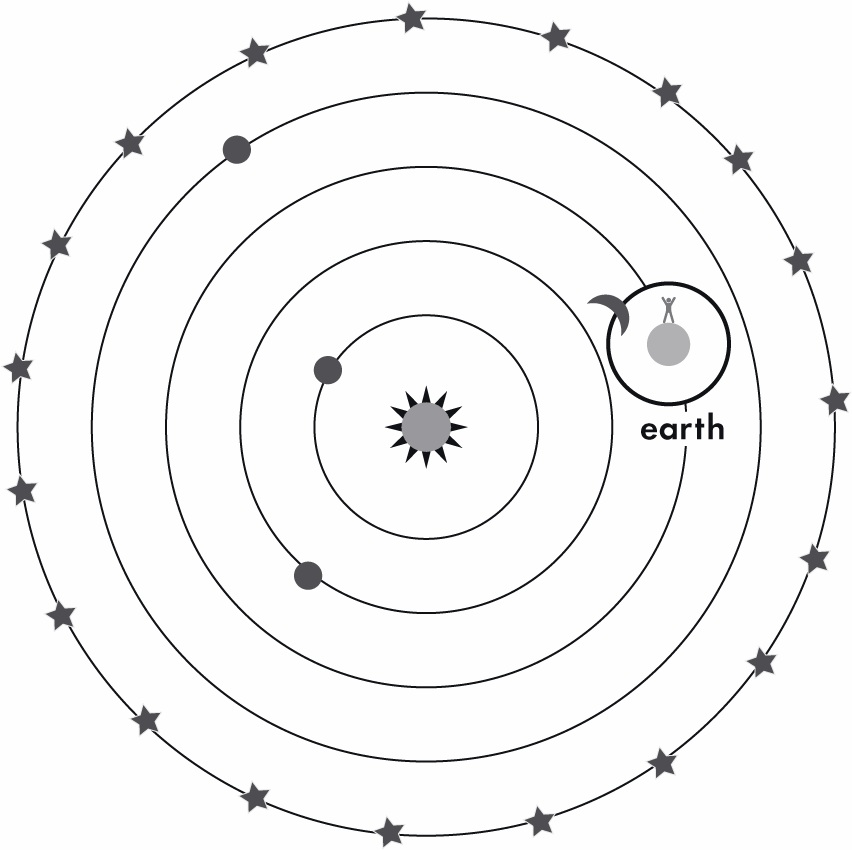
\includegraphics[width=.9\textwidth]{img/34.jpg}\\[12pt]
	\ec

   但是实际上有一个重要的区别。吸取了在古代就已经被考虑过的想法之后,哥白尼(Copernicus)了解到并且表明我们的地球不是行星舞会的中心,而是太阳在那里。我们的星球成为其中之一,高速地绕地轴和太阳的运转。

   我们认知的增长从未停止, 随着仪器的改良我们很快认识到我们的太阳系不过是其他众多太阳系的其中一个, 并且我们的太阳不过是一颗与其他恒星差不多的恒星. 一粒极微小的尘埃在一团由一千亿颗星星组成的磅礴星云---银河系之中。

	\bc
	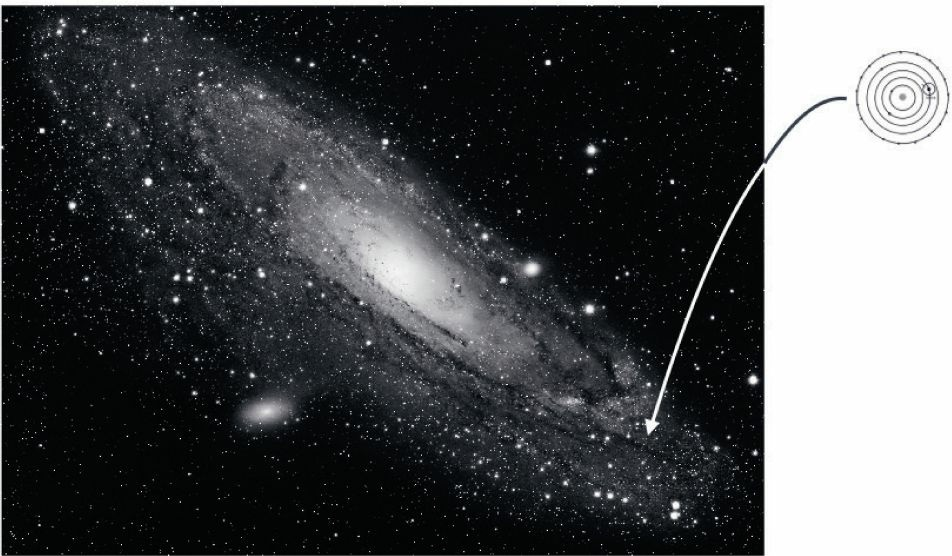
\includegraphics[width=.9\textwidth]{img/35.jpg}\\[12pt]
	\ec

   然而, 那些研究星云, 也就是群星之间发白的云状物, 的天文学家十九世纪三十年代所做出的精确测量表明, 我们的银河系也不过是, 由无数星系组成的绵延到人类最先进的望远镜所能观测到的最远处星空的巨大星系团中的沧海一粟. 人类的宇宙图景始终如一, 毫不停歇地扩张着. 

   以下插图并非是一副画, 它是哈勃太空望远镜拍摄的一副照片. 这张照片展现了一副比以往我们用最强大的望远镜所能看到的还要深的太空图景---如果用肉眼去观测, 这不过是黑色天空中极小的一块碎片. 透过哈勃太空望远镜 一片极其遥远的星尘展现在眼前. 图中每一个黑色的点都是一个包含了上千亿颗像我们的太阳这样的恒星的星系. 而在近几年的观测中, 我们发现这些恒星中的大部分都有行星绕其左右. 正因如此, 宇宙中应当有数千万亿亿的地球这样的行星. 而且这总发生在我们观测的任一方向上.

	\bc
	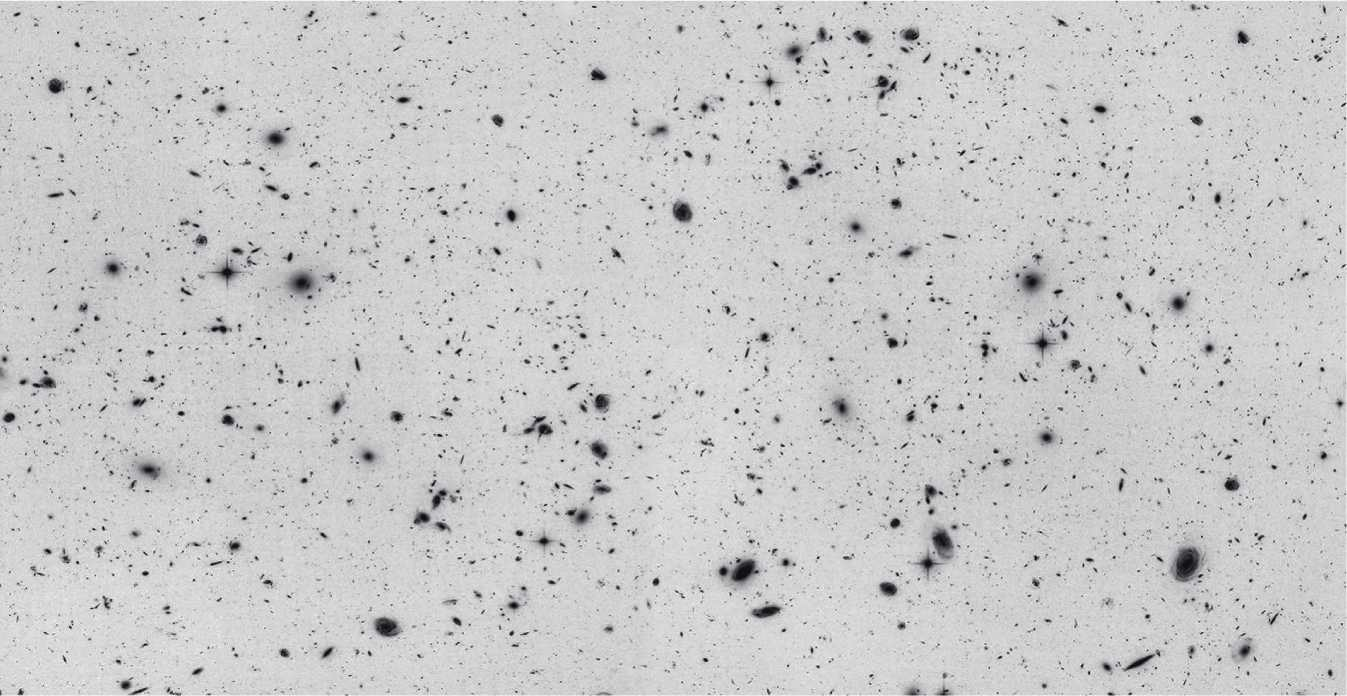
\includegraphics[width=.9\textwidth]{img/36.jpg}\\[12pt]
	\ec	
	\bc
	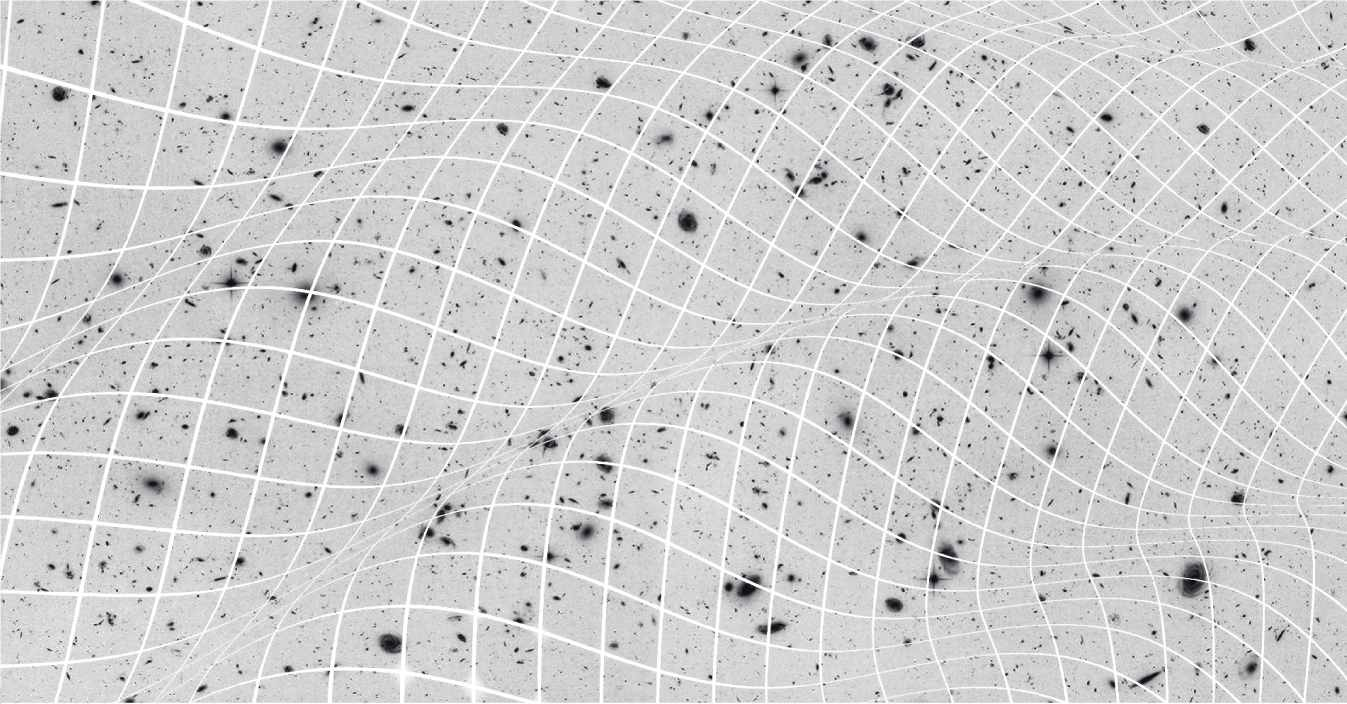
\includegraphics[width=.9\textwidth]{img/37.jpg}\\[12pt]
	\ec
	\bc
	
\includegraphics[width=.9\textwidth]{img/38.jpg}\\[12pt]
	\ec

\noindent

		\chapter{颗粒}
\indent

   在之前那一章被描述的宇宙中,光和事物都是运动的。光是由光子组成的,而光子是爱因斯坦假想出来的微粒。我们看到的每样事物都是由原子构成的,每个原子都包含着原子核和核外电子。每一个原子核又是由紧密连接的质子和中子组成的。质子和中子甚至都是由更小的微粒构成的,这种微粒被美国物理学家默里·盖尔曼称为“夸克”,而这个名词竟出自詹姆斯·乔伊斯的《芬尼根的守灵夜》中看似荒诞的一句话“为马克检阅者王三声夸克!”不管怎样,我们接触的每一件事物都是由电子和一些夸克组成的。

    在质子和中子中把夸克聚集在一起的力是由一种微粒产生的,物理学家没有一丝荒谬之感的称这些微粒为“胶粒”。

    电子,夸克,光子和胶粒都是我们身边空间中每件事物的组成成分。它们都是粒子物理中被研究的基本粒子。除了这些粒子之外,再加上例如聚集在整个宇宙中但和我们几乎没有相互作用的中微子,还有最近在日内瓦欧洲核子研究中心大型强子对撞机中发现的希格斯玻色子。但是它们的种类并不多,事实上少于10中。这些大量的基本材料就像在乐高积木中的砖块一样,组成了我们身边全部的真实的物体。

    这些粒子的性质以及他们是怎么运动的,是被量子力学研究的。这些粒子不像现实生活中的卵石水晶那样真实存在,但它们确实相当于相应领域中的量子,仅仅就像光子是电磁场领域的量子一样。他们是类似于法拉第和麦克斯韦领域中下层基本的激发体,微小移动的小波。他们按照量子力学中奇怪的法则消失和再现,在量子力学中,每一件事物都不是永恒存在的,每一件事物都是从一个作用变成另外一个作用。

    即使我们观察一个很小的空区域,并且在该区域中没有原子,我们仍然可以在某一片刻探测到涌动的粒子。真正的没有东西的虚空是不存在的。就像最平静的海洋中近观都会有微小的波动,所以形成世界的场都容易受到瞬时波动的影响,而且可以想象到它的基本粒子短暂的存在,并被这些运动持续的消灭和产生。

    这使由量子力学和粒子学说所描述的宇宙。我们已经到达了距离牛顿和拉普拉斯的力学世界很远的地方,在他们的世界里,冷石头可以永远的在几何上一成不变的空间中沿着漫长而准确的轨道上运动。量子力学和粒子实验已经告诉我们世界是一个连续的、不停涌动的东西;一个不停出现又消失的短暂的实体。是一系列的如同20世纪60年代嬉皮士世界一样的震动,一个由发生而不是事物组成的世界。

    粒子学说的细节是在20世纪50、60、70年代由那个世纪的像理查德·费曼和默里·盖尔曼一样最伟大的物理学家所逐渐建立的。这些建设工作引导向了基于量子力学的错综复杂的理论,并且有了一个“基本粒子的标准模型(the Standard Model of elementary particles)”这样一个非常浪漫的名字。“标准模型”是在20世纪70年代在进行一系列证实了所有预言的实验后总结出来的。它在2013年发现希格斯波色子后最终确立。

    尽管有一系列成功的实验,这个标准模型从未真正被物理学家们严肃对待。这个理论第一眼看上去破碎而缺乏通盘计划。它由一系列零部件毫无头绪地拼凑而成。若干个领域(确切的说为什么是他们?)通过若干力(为什么是这些力?)相互作用,它们由守恒量(为什么是这些量?)决定并展现出某种对称性(又一次,为什么是这些对称性?)。我们还离简单的的统一的方程,离量子力学很远。

   应用标准模型的方程组做预测,所使用的方法也是十分复杂而混乱的。如果直接使用这些方程,算出的每个被计算量都是无穷大的,结果是没有物理意义的。为了获得有物理意义的结果,不得不设想输入到方程组的常数本身就是无穷大的,来补偿荒谬的结果,使之合理化。这个复杂的和巴洛克风格的过程是在技术上被称为“重整化(renormalization)”。它确实生效了,但是使得那些追寻自然之简洁的人如鲠在喉。继爱因斯坦之后的二十世纪最伟大的科学家、量子力学的伟大建筑师、第一个重要的标准模型方程提出者,保罗·迪拉克,在他生命最后的时光里不断重复强调他对于目前状况的不满,得出“我们还没有解出这个问题”的结论。

   此外,标准模型的另一个显著限制也在近些年显现出来。几乎每一个星系天文学家都是在观察一大片物质云,它通过对恒星的引力而显示自己的存在,它也会偏折光线。我们虽然能观测到它的引力效应,但是由于不能直接观测到它所以不能确定它的组成。为此提出了大量的假说,但没有一个是有效的。我们清楚的是那里一定有东西,但我们不清楚它是什么。现在,我们都把它称作“暗物质”。证据表明,它不能被“标准模型”所描述,否则我们就能看到它了。它是一种原子、中微子、光子等等之外的存在。

   一点也不令人奇怪的是,天上和地上的事物比我们物理或者哲学所能设想到的要多。充满宇宙的无线电波和中微子,我们也是近些年来才相信它们的存在的。如今对于物质世界,标准模型包含了所有理论之精华,它的所有预言也都得到了确认,除了暗物质,它能很好的描述已知宇宙的方方面面,引力也被广义相对论描述为时空的扭曲。

   前面我们已经提出了几种只能被实验所驳倒的理论。19世纪70年代有人提出的一个完善的理论并赋予了它一个专门的名字——SU5。举个例子,这个理论用一个更加简单和优雅的结构替代了标准模型中的无序的等式。这个理论预测一个质子有一个特定的可能性会衰变,转化成电子和夸克。人们建造了大型机械来观察质子的衰变。物理学家们奉献了他们的一生来寻找一个可观察的质子衰变。(你不能一直盯着一个质子看,因为质子的衰变需要很长的时间。应该用成吨的水进行实验并用敏感的传感器来检测是否发生衰变。)但是,唉,至今还没有观察到任何质子衰变的发生。SU5这个美丽的理论,尽管有着十分优雅但它并不被上帝所喜爱。

   这个故事也许正在借着被称作“超对称”的理论重复着。“超对称”理论预测了新一级别的粒子的存在。在我的职业生涯中已经听过很多对这些粒子即将出现充满信心的同事的言论。一天,一个月,一年甚至十年过去了——但是超对称的粒子仍然没有出现。物理学不只是成功者的历史。

   所以,现在我们还要坚持使用标准模型。标准模型也许不是很优雅,但是它在形容我们身边的世界时工作的效果很棒。那么谁知道呢?也许通过更深入的检查它并不是一个缺乏优雅度的模型。也许是我们没有学会从一个正确的角度来看待这个模型。从这个角度来看我们能发现它所隐藏的简易性。目前这是我们关于这个问题所知道的一切:

   许多种类的基础粒子,在存在与不存在之间持续的振动和波动,甚至会蜂拥在一个看似没有任何事物的空间内。无穷多个粒子聚合在一起就像宇宙字母表的文字一样告诉我们星系的,数不胜数的星星的,阳光的,山峰的,森林和成片的谷地的,聚会上年轻人们的笑脸的,镶满星星的夜空的久远历史。

\noindent

		\chapter{粒空间}
\indent

   尽管依旧艰难依旧困惑依旧有解决不了的问题,但我已经比我们之前所能描绘的物理现象有了更清晰的轮廓。所以,按理说我们应该满意,但是我们还不能。

   在我们对物理学世界理解的核心中有一个悖论。二十世纪已经遗留给了我们两大物理学珍宝:相对论和量子力学。相对论推动了宇宙论的发展,还有天体物理学,以及引力波,黑洞等很多其他方面的研究的发展。量子力学为原子物理,核物理,基本粒子物理,凝聚态物理以及许多许多方面提供了理论根基。两个理论的应用,是我们今天科技的基础,并已经改变了我们的生活方式。但这两个理论至少在现在的形式下一定不都是对的,因为它们相互矛盾。

   一个早晨听了相对论的演讲,下午听了量子力学的演讲的大学生如果得出,他的老师是傻子,或者这两个教授已经至少一个世纪都没交流过的结论,是可以被原谅的。在早晨,这个世界是被卷曲的但依旧处处连续的。在下午,这世界就是一个平的空间,处处有量子能级。
   一个大学生早晨听了相对论的演讲,下午听了量子力学的演讲,如果他得出,他的老师是傻子,或者这两个教授已经至少一个世纪都没交流过的结论,是可以被原谅的。在早晨,这个世界是被卷曲的但依旧处处连续的。在下午,这世界就是一个平的空间,处处有量子能级。

   悖论在于这两个理论在理论实践中都发挥的相当完美。自然正使我们表现的像一个老年法师去调解两个争论不休的男人。已经听完了第一个人的论述,法师说:“你是对的。”,第二个人坚持要陈述观点,法师听完他表述之后说到:“你也是对的。”在隔壁屋里,偶然间听到这谈话的法师的妻子说道:“但他们不可能都是对的啊。”法师沉思了,并且在得出“你们都是对的”之前来回纠结着。

   五湖四海的理论物理学家正费力的尝试去解决这个问题。他们的研究领域叫做“圈量子引力论”,它的目标是去找一个理论,可以说是一个方程,但是可以包含所有的这个世界的可发生的现象,同时它也能解决现在这个精神分裂症般的理论。

   这已经不是第一次物理学家发现他们面对两个高度成功但明显相互矛盾的理论。过去的对此的努力使我们高速的认识了我们所在的世界。牛顿靠整合伽利略的抛物线和开普勒的椭圆发现了万有引力定律。麦克斯韦考整合电学理论和磁场理论发现了电磁场方程组。爱因斯坦凭借着解决明显的电磁学与力学的冲突,提出了相对论。当一名物理学家发现两个成功理论的相矛盾之处会非常高兴,因为这是一个绝佳的机会。我们能依靠思考从这两个理论中学习到的可兼容的世界建立一个概念性的框架吗?

   在这里,学术前沿地带,超越知识的边界,科学变得更加美丽——在幼嫩的想法,直觉和尝试的锻造中变得炙热,耀眼。这也发生在条条道路的兴废中,在热忱中,在想象尚未被想象事物的努力中。

   二十年前,在这些未知领域浓雾很重。然而今天曙光已经出现。它已经激起人们的热情和乐观。然而这里不止有一条道路,因此也不能说这个问题已经解决.多重道路产生了争议,但这些争论是健康的:直到迷雾完全散去,有批判和反对的观点就是有利的。尝试去解决这个问题之一的龙头理论的研究方向叫做“圈量子引力论”。现在这个方向被在各个国家的很多的精良的研究小组所信奉。

   圈量子引力论是整合广义相对论和量子力学的努力。因为它仅采用了理论已有的假设并适当地改写使之兼容。所以它是谨慎的。但它的结论是较为激进的:一个关于我们观察现实结构方式的更深远的改变。

   这个想法是简单的。相对论已经告诉我们,空间不是一个惰性的长方盒,而是一种动态的东西:一种包含我们在内的,巨大的可移动的,可以被压缩,卷曲的蜗牛壳。另一方面,量子力学已经告诉我们一切场都是由量子组成的,并且有良好的颗粒状的结构。紧随而来的结论就是,物理空间也是由量子组成。

   圈量子引力论的中心结论确实指出空间不是连续的,而且其不是无限可分的而是由微小粒子组成或者说是“原子空间”组成。它们是极小的:比最小的原子核的一亿亿分之一还要小。这个理论描述了这些“原子空间”在数学上的形式,并提供了决定它们演化方式的方程。这些方程被称为“圈”,或者环,因为他们相互联系,组成了网状结构。这种网状结构像精细编织的巨大锁子匣一样,编织出了空间材质。

   那这些空间量子在哪呢?哪也不在。它们不存在于空间,因为它们本身即空间。空间靠连接这些独立的引力量子而被创造。又一次,世界看起来,相比于是关于物体的,更像是关于交互关系的。

   但是这是该理论的第二个结论,也是最极端的结论。正如连续的空间包含着物体的想法不存在了,所以基本的原始的与物体无关的时间流也不存在了。描述空间颗粒和物质的方程不再含有时间变量。但这不意味着任何事物都是静止的和不变的。正相反,这意味着改变是无处不在的——但是基本过程不能够被排列为一个普通的“极小瞬间”的序列。在非常小的粒空间尺度上,自然的舞蹈不能按照管弦乐团指挥官手中指挥棒的节奏,在每一个节拍中:每个过程的舞蹈都独立于其旁边的舞者有他自己的节奏。时光流逝是世界的内在规律,它诞生于世界中的两个量子事件之间,量子事件包含着世界并且它们自己就是时间的来源。

   在这个理论描述下的世界因此变得和我们所熟悉的世界更加遥远。这里不再有空间包含世界,也不再有时间中发生事件。这里只有基本进程。在进程中,空间和物质量子不断相互影响。我们身边连续的空间和时间的幻象其实是对集群的基础过程的混乱的认识。就像风平浪静的阿尔卑斯湖实际上包含无数快速舞蹈的微小水分子。

   通过甚强的放大镜,用考察极端的特写镜头,在我们第五章的倒数第二图片会展示空间的颗粒结构。

   有可能实验验证这个理论吗?我们思考着尝试着,但是还没有实验的验证。无论如何,有一些不同的尝试。

   这些尝试中的一支派生出了黑洞的研究。在天空中我们已经可以观察坍缩恒星形成的黑洞。这些恒星被自身质量压碎,向自身塌陷,以及从我们的视野中消失。但是它去哪了?如果圈量子引力论是正确的,物质不可能真正探索到一个无穷的点上,因为不存在只有有限大小的宇宙块。在自身的重量下坍缩,物质一定会变得更加稠密,直到某个时刻,在这个时刻量子力学一定会产生反作用的平衡力。

   在假设的恒星生命的最后阶段就是人们所知的“普朗克星”。在这一阶段中时空量子涨落平衡了物质自身重量。如果太阳停止燃烧,形成一个黑洞,黑洞直径将会有约一点五公里。在这个黑洞中心,太阳的物质将会继续探索,最终成为普朗克星。它的尺度就和那些原子的尺度差不多。太阳全部的物质被压缩进一个原子的空间:一个普朗克星应该是由这样极端状态的物质构成的。

   普朗克星不稳定:一旦压缩到极限,它就会反弹,开始重新膨胀。这会导致一次黑洞爆炸。就像一个坐在黑洞中普朗克星上的假设观察者,这个过程将会是一个发生得极快的反弹。但是对于这个观察者,那些在黑洞外面的人时间不会以同样的速度流逝。同样的理由,在山上时间会比在海平面流逝得更快。除非她以外,因为极端条件,时间片段的差别是巨大的,并且对于恒星上观察者极快的反弹,对外面的人来说显得是在很长一段时间发生的事。这就是为什么我们观察黑洞总是在相当长时间中保持不变:黑洞是以看起来极端缓慢的动作正在反弹。

   有可能在第一批宇宙黑洞形成的大熔炉中,黑洞中的一部分正在爆炸。我们如果是正确的,就很可能观测到它们爆炸所激发出的,以来自太空高能宇宙射线形式的信号。这也允许我们观测和测量量子引力主导现象的直接效应。这是一个大胆的想法——它有可能失效,比如可能在原始宇宙没有形成足够多的黑洞,能让我们今天来探测它们的爆炸。但是这个信号的探索研究已经展开。

   这个理论的另一个结论,也是最壮观的结论之一,关系到宇宙的起源。我们知道怎样重建我们行星的历史,直到最初的,它还很小的时期。但是在那之前呢?对的,圈理论的方程允许我们回溯得更远,重建它的历史。

   我们可以发现当宇宙还极度压缩的时候,量子理论产生了斥力,导致了巨大的爆炸,“大爆炸”或者事实上是“大反弹”。事实上,我们的世界可能诞生自从,反弹之前的一个宇宙。这个宇宙在自身重力下坍缩到一个极小空间,正要重新膨胀,从而成为我们观测到的,身边正在膨胀的宇宙。

   在这个反弹的瞬间,宇宙坍缩进一个坚果壳内,是真正的量子引力的领域:时间和空间同时消失了,世界被溶化成一团集群的概率云。然而我们的方程依然能描述这个概率云。第五堂课的最终图景被转换成下图:

   我们的宇宙可能诞生自先前阶段的反弹,并经过一个既没有空间也没有时间的中间阶段。

   物理打开了一扇窗,从中我们可以看得很远,我们所见将会一直震惊我们。我们意识到,自身充满偏见,自身对世界的直觉图景也是偏颇的,狭隘的,也是不恰当的。世界不是平坦的,也不是静止的。世界将在我们眼前继续变化,随着我们逐渐能够将它看得更广阔,看得更清晰。如果我们尝试整理我们在二十世纪关于物理世界的所学,线索将会指向和我们对物质,空间和时间的直觉理解有深刻差异的事物上。圈量子引力是一个破译这些线索的尝试,也是看向更远的一点距离得尝试。

\noindent

		\chapter{概率、时间与黑洞的热}
\indent
   除了我已经讨论过的描述世界基本组成的主要理论以外,物理学仍然有一大堡垒与其他理论有所不同。一个简单的问题意想不到地产生了它:“什么是热?”

   截止到19世纪中叶时,物理学家们尝试着把热理解为一种叫做“热质”的流体;或者是两种流体:一种热的,一种冷的。这个想法后来被证明是错误的。詹姆斯·麦克斯韦与奥地利物理学家路德维希·玻尔兹曼最终理解了热的本质。他们的解释十分奇特出众而影响深远——并且带领我们进入了很大程度上尚未被探索的领域。

   他们的研究表明一个有热量的物体并不包含任何热质。它不过是由运动更剧烈的原子们所组成。原子与分子以及束缚在一起的小型原子团不停地运动着。它们飞驰着、振动着、碰撞着……冷空气是由运动更缓慢的原子——或者说,分子——所构成的。而热空气是由运动更激烈的分子构成的。这个理论简洁而美丽,但却不止于此。

   正像我们所熟知的那样,热量总是从热的物体传向冷的物体。比如一个放在一杯热茶中的冷茶匙会变热,而我们不在气温低时多穿一点就会很快丧失我们身体的热量并感到寒冷。那么为什么热量会从热的物体传向冷的物体而不是相反呢?

   这是一个关键的问题,因为这关系到时间的特性。在热量交换不发生或不明显的每个案例中,我们都能观察到系统的将来与过去十分相似。例如,热与太阳系中行星的运动几乎完全不相干,而事实上这样的运动可以反向的方式同等发生而不违反任何物理法则。然而,只要有热的存在,未来就不会与过去相同。比如说在没有摩擦的情况下,摆锤会不停地摆下去。如果我们将其拍摄下来并将录像倒放,我们将会发现这运动是完全可能的。但是如果存在摩擦,那么摆锤将会极轻微地传热给它的支撑物并失去能量、缓慢减速:摩擦生热。而且我们能立刻分辨出未来(沿摆锤减速的时间方向)与过去的不同。我们从未见过一个从静止状态开始通过从支撑物吸收热进而摆动的摆锤。未来与过去的差别只有存在热时才会出现。这种基本物理现象借助热量由热的物体导向冷的物体实现了未来与过去的分离。

   那么,再一次的,为什么随着时间流逝热从热的物体传向冷的物体而不是相反呢?

   玻尔兹曼发现了这个简单得令人惊奇的原因:纯粹的概率。

   玻尔兹曼的想法十分微妙,他引入了概率的理论。热并不是由于一条绝对的定律决定了它是由热的物体传向冷的物体的:热有如此的表现只是因为更大的可能性。这背后的原因是当一个处在较热物体中的快速移动的原子撞到一个较冷的原子时会更有可能传递给后者些许其自身的能量而不是相反。碰撞传递了能量但每次碰撞却并不同等地分配着能量。因此相互接触的物体的温度才会趋于一致。一个与较冷物体接触的较热物体是不可能通过它们间的联系而变得更热的:而这是极其不可能的。

   概率论向物理学核心的引入与在解释热动力学的基础方面的应用首当其冲地被认为是十分荒唐的。当时经常会看到没有人认真对待玻尔兹曼。1906.9.5,他在Trieste附近的Duino上吊自杀,永远也没有机会目睹他的理论收到普遍的承认。

   在第二课中我将量子力学如何预测每一小块物体的运动通过概率联系起来。这也将概率论放进了理论中央。但是玻尔兹曼考虑的关于热的本质的概率论与之有所不同。热力学中的概率在某种意义上与我们的无知紧密相连。

   也许我并不知晓有关概率论的相关内容,但我仍然可以确定一个对某事的或较大程度的可能性。例如,我不知道明天马赛港会下雨,也不会知道是晴天还是下雪,但是马赛港8月份下雪的概率很低。同样,对于大多数物体,我们有些许了解,但不完全知晓关于它们的状态的一切,我们只能根据概率进行预测。想象一个充满空气的气球。我可以测量它:测量它的形状、体积、压强、温度……但是气球内部的空气分子在其中快速移动,我不知道它们的确切位置。这阻止了我精确地预测气球的行为。例如,如果我解开这个结的封条,让它去它会缩小闹,冲和碰撞在一路,我将无法预测。因为我只知道它的形状、体积、压力和温度。气球的运动取决于内部分子的碰撞。然而,即使我不能准确地预测每一件事,我也能预测一件事或另一件事发生的可能性。例如,气球几乎不可能会飞出窗外绕着远处的灯塔旋转,然后降落到我的手上。有些时间更可能发生,而其他时间更不可能。

   同样,分子碰撞时热从较热的物体传递到较冷的物体的概率可以计算出比热向热物体传递的概率大得多。

   解释这些事实的科学分支被称为统计物理学。它的一个起自玻尔兹曼的成果解释了热和温度的概率性——那就是热力学。

   乍看之下,我们的无知昭示了物质的属性的想法似乎并不合理:热茶中的冷茶匙变热和气球被释放乱飞时。我们知道或不知道的事实与物理定律有什么关系?这个问题是合理的;而它的答案十分微妙。

   茶匙和气球的行为必须遵循完全独立于我们认知的物理定律。它们行为的可预测性或不可预知性与它们的精确状态无关;而与其相互作用的属性的有限集有关。这组属性取决于我们与茶匙或气球相互作用的具体方式。概率并不是指物质本身的进化。它涉及到与我们交互的那些特定数量的演变。再次地,我们用来组织世界的概念的深刻的本质关系显现了。

   冷茶匙在热茶中加热是因为茶和勺子相互作用。我们通过有限数量的变量,在无数的变量影响下,描述它们的行为。这些变量的值不足以准确预测未来的行为(比如气球的飞行),但足以预测勺子温度变化的最大可能性。

   我希望读者没有丧失对这些精妙的辨别的注重……

   现在,在二十世纪热力学(即关于热的科学)和统计力学(即不同运动的概率的科学)的课程已经扩展到了电磁和量子现象。然而,包含引力场的扩展被证明是有问题的。重力场在加热时的行为如何,仍是一个尚未解决的问题。

   我们知道在加热的电磁场中会发生什么:例如,在烤箱中有一种热电磁辐射可以烹饪馅饼,我们知道如何描述它。电磁波振动,随机共享的能量,我们将这团光子想象为在一个热气球中运动的分子。但是什么是热引力场呢?

   正如我们在第一节课中看到的,引力场即是空间本身。它影响时空。因此,当热量被扩散到重力场时,时间和空间本身必须振动……但我们仍然不知道如何描述这个井。我们没有方程来描述热时空的热振动。什么是振动时间?

   这些问题把我们带到时间问题的核心:时间的确切流向是什么?

   这个问题已经存在于古典物理学中,哲学家们在第十九、第二十世纪强调了这一点,但它在现代物理学中变得更为尖锐。物理学用公式来描述世界,它告诉事物如何随时间的变化而变化。但我们可以写公式,告诉我们如何在关系到他们的位置的不同,或是食物的味道关于黄油的变量函数。但时间似乎是流动的,而黄油或空间的位置并不流动。差别来自哪里?

   提出问题的另一种方法是问自己:什么是“现在”?我们说,只有现在的事物存在:过去不再存在,未来也不存在。但在物理学中,没有什么与“现在”的概念相对应。比较“现在”和“这里”。这里指定说话者的位置:两个不同的人在这里指向两个不同的地方。因此“这里”是一个词,它的意思是什么取决于它在哪里说。这种话语的术语是“索引”。“现在”也指说出这个词的瞬间,也归类为“索引”。但是没有人会梦想说“存在于这里”,而不存在于此的事物并不存在。那么为什么我们说“现在”存在,而其他事物不存在?“现在”是客观存在的东西吗?“流动”,使事物“一个接一个地存在”,还是只是主观的,像“这里”?

   这似乎是一个深奥的心理问题。但在现代物理学中已成为一个热点问题,因为狭义相对论表明,“现在”这个概念也是主观的。物理学家和哲学家得出的结论是,对于整个宇宙来说,一个普遍存在的概念是一个幻象,宇宙的“时间流”是一个不起作用的概括。当他的意大利朋友Michele Besso去世时,爱因斯坦写了一封感人的信给米歇尔的姐姐:“米歇尔已经一点点在我面前离开了这个陌生的世界。这意味着什么。像我们这样相信物理的人,知道过去、现在和未来之间的区别只不过是一种顽固的幻觉。

   幻想与否、是什么向我们解释了时间的流动与消逝呢?时间的流逝对我们所有人来说都是显而易见的:我们的思想和我们的语言都存在于时间之中;我们语言的结构需要时间——一件事物“是”或“曾是”或“将来是”。可以想象一个没有色彩的世界,没有物质,甚至没有空间,但很难想象一个世界没有时间。德国哲学家马丁·海德格尔强调了我们的“时间的栖居”。海德格尔对原始世界的描述是否有可能在世界的描述中消失?

   有些哲学家是海德格尔最忠实的追随者,他们得出结论:物理学不能描述现实的最基本的方面,并将其视为一种误导性的知识形式。但很多时候,在过去我们已经意识到,我们眼前的直觉并不精确的:我们将仍相信地球是平的且围绕太阳的。我们的直觉是在有限的经验基础上发展起来的。当我们向前看得更远一点时,我们发现世界并不像我们想象的那样:地球是圆的,开普敦的人脚高而头低。相信眼前的直觉,而不是理性、谨慎和聪明的集体检查,那就不是智慧:这是一个老人的假设,他拒绝相信他村外的伟大世界与他所知道的世界是不同的。

正如我们所看到的那样生动,我们对时间流逝的体验不需要反映现实的一个基本方面。但如果它不是根本性的,我们对时间流逝的生动体验,它来自哪里?

   我认为答案在于时间和热量之间的紧密联系。只有在有热的时候,过去和未来才会有区别。热与概率有关,而概率又与我们与世界其他地方的相互作用不符合现实的细节有关。时间的流动是从物理学中产生的,而不是在对事物的精确描述的背景下。它出现在统计和热力学的背景下。这可能是时间之谜的钥匙。现在不在客观上比“这里”的存在是客观存在的,但在微观世界的相互作用提示时间的现象出现在一个系统(例如,我们只有相互作用)通过无数的变量中。

   我们的记忆和意识是建立在这些统计上的现象。一个假设的超感官是不会有“流动”的时间:宇宙是一个单块的过去,现在和未来。但由于我们意识的局限性,我们只能觉察到世界的模糊景象,并活在时间之中。借用我的意大利编辑的话:“不明显比明显的要多得多。”从这有限的、模糊的焦点中,我们可以看到时间的流逝。懂了吗?不,它不是。还有很多东西需要理解。

时间处于引力、量子力学和热力学交叉点引起的问题的中心。我们仍然有一系列问题处在黑暗之中。如果我们可能已经开始了解量子引力,就会发现它结合了这三个谜题中的两个,但我们还没有一个理论能够把我们对世界的基本知识的三个部分结合起来。

   解决这个问题的一个小小的线索来自于物理学家Stephen Hawking完成的计算,这位物理学家虽然身体状况不好,但他却始终借助着机械的辅助勉力工作着。

   霍金利用量子力学成功地证明黑洞总是“热的”。它们像火炉一样散发热量。这是对“热空间”性质的第一个具体指示。从来没有人观察到这种热,因为它在目前观测到的黑洞中是微弱的,但霍金的计算是令人信服的,它以不同的方式重复,黑洞的热的现实被普遍接受。黑洞的热是物体上的量子效应,黑洞是自然界的引力。它是空间的单个量子,空间的基本粒子,振动分子,加热黑洞表面并产生黑洞热。这一现象涉及到量子力学、广义相对论和热科学的三个方面。黑洞的热就像物理学的Rosetta Stone,使用三种语言–量子、引力和热力学。它仍在等待我们来揭示时间的本质。

\noindent

		\chapter{最后:我们自己}
\indent

   从深空的结构到所认知的宇宙边界我们已经遨游了如此遥远了。在这之后,在结束这系列课程致前,我想回归到我们这个主题上来。

   当代物理描绘出一幅世界的伟大壁画。在这物理学家所绘制的壁画中,我们作为感知者决定者,能自由表达自己情感的人类,扮演了一个怎样的角色呢?如果世界是一群转瞬即逝的空间和物质的量子,如同一个空间和基本粒子的巨大拼图,那我们是什么?我们也仅仅是由量子和粒子构成的吗?如果是这样,那我们全部都能证明的,个体存在感和独特的个性,又是从何得来的呢?以及我们的价值,我们的梦想,我们的感情,我们的个体知识又是什么?在这个漫无边界又光芒无限的世界中,我们又是什么呢?

   我甚至不能想象用这简单的篇幅去真正完美回答这样一个深奥的问题。这是一个艰深的问题。在当代科学的巨大图景中,有很多我们暂时无法理解的事物。其中,我们最不能理解的一个就是我们自己。但若是回避或者忽略这个问题,我想,我们会遗漏某些关键性的事物。我已经着手于展示科学之光下的世界是何面貌,以及,作为这个世界的一部分的我们的面貌。

   我们,人类,是第一个也是最重要的,观察世界的主体;也是我所尝试组合的显示照片的集体作者。我们是传递图像、工具、信息和知识的交换(本书就是一个例子)网络中的结点。

   但是我们也是我们所感知的世界的一个整体部分;我们不是外部的观察者。我是置身其中。我们对世界的认知来自其中。我们由相同的原子,和像在山中松树和群星间交换的相同的光信号所组成。

   随着我们知识的增长,我们已经认识到我们只是宇宙的一部分,那么小的一部分。

   几个世纪以来,尤其是在上个世纪,这一点变得越来越明显。我们曾经相信我们是在宇宙中心的星球上,其实我们不是。我们曾认为我们是一个特别的存在,一个独立于动植物的种族,其实发现我们是和身边一切生物共同祖辈的后代。我们和蝴蝶落叶松有着共同的祖先。我们只是唯一一个长大了的孩子,唯一地认识到世界没有像小时候那样围绕着孩子们。他们终会认识到我是众生中的一员。参照他们,参照其他的事物,终将了解我们是谁。

   在德国唯心主义的全盛时期,谢林大概认为人性代表了自然的顶峰,最高点,在此现实意识到了自己。今天,从我们现在对自然世界的知识提供的视点看,谢林的想法只会让我们会心一笑。即使我们与众不同,也只是每个人感到自己不同这般。这仅仅如同每个母亲对于她的子女这般的不同。但是对于自然的其余部分,显然就不是这样了。

   在巨大星河中,我们偏居一隅;在构成现实的无限的不同样式的蔓藤花纹之中,我们只是无数我们这样点缀的其中一个。

   我们所构建的宇宙图景在我们思维空间中与我们俱生。我们能够重建并用浅薄手段能够理解的事物,如同图片,和我们作为一部分的现实世界之间,存在着无数的马赛克筛子:我们的无知,我们感知和智慧的有限。我们自然作为主体,作为特定的主体,这个恰恰相同的条件。

   这些条件,康德设想的是那样普遍——从中推出自欧几里得空间甚至到牛顿力学的自然,而因此注定是先验的。无论如何,它们不是。它们是我们种族精神演化的结果,是在连续的演化中的。我们不仅认识到,也渐渐认识到去改变我们理念框架,以使之适应于我们所认知。并且我们尽管缓慢犹豫,但一直在学习去认识到的,正是我们作为部分的现实世界的自然。我们建构宇宙的图景活在我们心中,在理念的空间中;但是他们也或多或少描述了我们所属的宇宙。我们为了更好地描述这个世界而遵循线索。

   当我们谈起“大爆炸”或者空间结构的时候,我们正在做的不是人们千百年来在篝火讲述自由奇幻的故事的延续。它是别的东西的延续。在一天的第一缕光中,看着羚羊在大草原尘土中留下的痕迹,仔细观察,从现实的细节中剔出,寻求无法直接看见,但可以追寻踪迹的东西。在我们总会犯错因而时刻准备在新踪迹出现时转向的意识中,但也同时在认识到如果我们做得足够好,我们最终会正确并找到我们一直所寻找的猎物。这就是科学的自然。

   在这两类人类活动——发明故事和按图索骥——中的困惑,就是在我们当代文化下展现出的对科学的不解和怀疑。这个分歧是个微妙的分歧:破晓时被猎捕的羚羊还未从在夜时故事会中的羚羊众神中远远剔除。

   二者的边界是互通的。神话滋养着科学,科学滋养着神话。但是,一旦我们发现了可以吃掉的一只羚羊,知识的价值将会留存。

   我们的知识持续的映射着世界。它或多或少,但的的确确反映了我们所栖息的世界。我们自身和世界的这个沟通,不是我们和自然的其余部分间的区分。一切事物都一刻不停地相互作用着,在作用中每个事物都产生着与其作用过的事物的痕迹:在这个意义上一切事物都一直在相互交换着信息。

   一个物理系统对另一个系统的信息对其而言没有任何精神性或者主观性:他仅仅是物理决定的一者和他者间的联系。一滴雨包含了天空中出现云的信息;一束光包含了其发射源的颜色;一个时钟有着一天的信息,风承载了将至的暴风的信息;流感承载了我鼻子易感性的信息;我们细胞中DNA包含了一切我们基因编码的信息(在我和父母相像的意义上);以及我大脑充满我经历所积累的信息。我们思维的原始面目就是一个极端富集的信息。而且它在不断积累,交换并且娓娓道来。

   即使我中心供热系统的恒温器也“感知”并“知晓”我家的大气温度,并且拥有他的信息,可以在够热的时候自己关掉。所以,在温暖并自由决定关闭加热与否上,那恒温器的“感知”和“知晓”与我们的“感知”和“知晓”区别是什么?也“知晓”我的存在吗?到底自然中怎样的信息交换产生了我们和我们的思维?

   问题是开放的,有着无数在讨论之中的解答。我相信这是科学最有趣的前沿。在这里主要的过程就是关于被创造。今天新的工具允许我们观察啊活跃大脑的活动,并且能够视听化地定位高度错综复杂的网络。正如2014年新闻所宣布的首个哺乳动物的大脑结构彻底(中观)详细定位被完成。对结构的数学形式可以对应于意识的主观体验的观点现在正在讨论中。这不仅仅是被哲学家讨论着,也正在被神经学家讨论着。

   举一个奇妙的例子,朱利奥·托诺尼——一位工作在美国的意大利科学家——发展了一个数学理论,被称为“积分信息理论”。它试图定性特征化具备意识的系统的必要结构:作为例子的一个方法是,描述我们在清醒(意识)和无梦睡眠(无意识)间到底发生了什么变化。它仍然还在发展阶段。对于我们意识到底如何形成,我们仍然没有令人信服的,已经建立的答案。但对我而言迷雾渐渐清晰。

   有一个问题,特别是关于我们自己,常常让我们困惑的问题:如果我们的行为仅仅是预定的自然法则,那我们决定的自由意味着什么呢?我们自由感和如同我们现在所了解的,世间万物运行的严谨,这二者之间有没有可能不存在一个矛盾呢?我们内在可能有没有,这样一个东西,让逃离自然的规律,让我们用自由思考的力量去扭曲和偏离自然规律?

   好吧,答案是否。这里没有能让我们逃离自然法则的东西。如果我们内在存在着可以违背自然的某种事物,到现在我们可能早就发现它了。我们内在没有和事物的自然行为存在矛盾之处。整个现代科学——从物理到化学以及从生物到神经科学——只是仅仅证实了这种观察。

   对这种困惑的答案到处都是。当我们说我们是自由的并且我们可能自由是真的,这就意味着我们如何行为是由我们内部,在大脑中发生的事物所决定的,而不仅仅是外部因素。是自由的不意味着我们的行为不受自然法则决定。这只是意味着它受我们大脑中活动的自然法则所决定。

   我们自由决定是由我们大脑中数亿神经元间的,丰富和流动的交互结果所决定:它们是自由的。从这些神经元所能允许和决定的交互的意义上来说是这样的。这可以意味着当我作决定,是“我”真正决定了?是的,当然。因为下面这个问题显得很荒诞。“我”到底能不能做与我整个复杂神经元所决定的不同的事物:这两者,如同荷兰哲学家巴鲁奇·斯宾诺莎在十七世纪所无比清晰理解的一样,是完全相同的。

   单独的“我”和“大脑中的神经元”都是不存在的。它们是相同的东西。一个个体,就是一个进程:复杂,高度集中。

   当我们说人类行为不可预测的时候我们是对的,因为预测太过复杂,尤其是被我们自己预测。我们强烈的内在自由感,如同斯宾诺莎敏锐观察到的,来自于我们关于自生的想法和图景相比于我们内在发生的细节的复杂事物来说是远远地更加粗略的。我们就是我们自己眼中无尽惊奇的源头。

   我们大脑中有数百亿神经元,像星系中的群星那般多的。这些神经元甚至有着天文般更多的连接和可能组合。通过这些组合神经元可以相互作用。我们不可能意识到这全部。“我们”是由这复杂整体组成的进程,而不是其中使我们有意识的一小部分。

   决定的“我”就是自我反思构成(某种意义上仍然不完全清晰但是我们已经开始了解)的“我”;也是在世界中自我表达构成的“我”;也是自身理解为置于世界背景下的一个可变化的观察点的这种想法构成的“我”;也是大脑中处理信息组成表达的宏大结构构成的“我”。当我们已经感受到“这就是我”在做决定的时候,我们就是正确的。如果不是那又是别的谁呢?

   如同斯宾诺莎所维持的,我就是我的身体和发生在我心脑中的事物,也是在于我而言的他们的巨大的不可思议的巨大复杂性。

   涉及到这些篇幅的,我所拥有的科学的世界图景,不会,和我们对自己的感知相不适。它也不会和道德或者心理学术语下我们的思维相不适,也不会和我们情绪和感受相不适。世界是复杂的,我们用不同语言去描述它,每个语言都与我们正在描述的进程相适宜。每个复杂进程可以在不同语言中和在不同层次下被定位和理解。这些丰富的语言交互相织也相互促进,就像这些进程本身一样。在我们对大脑生化学理解之下,对心理的研究变得更加复杂。使我们活跃的热情和情绪滋养着理论物理的研究。

   我们的道德价值,我们的情绪,我们的爱,不再那么缥缈地作为自然的一部分,缥缈地和动物所共享共享或者缥缈地被我们种族百万年来潜移默化的演变所决定。他们只是我们创造的复杂现实世界。我们的现实就是眼泪和欢笑,感恩和无私,忠诚和背叛,过去萦绕我们的,和平静。我们的现实世界有社会,有音乐激发的情绪,由我们共同构建的寻常知识组成的富集的交织的网络。所有的这些只是被我们描述的自同为“自然”的一部分。我们是自然的一个整体部分。我们就是一个有着无穷无尽变量的表达式中的自然。这就是我们从对于世界事物不断增长的认知中所学会的。

   使我们明确成为人类不表示我们和自然的分离;这是自同自然的一部分。这是发生在我们星球上的,在组合的无尽表达下,通过相互影响和部分之间信息和关联的交换,是这样的形式,谁知道有多少和其他的非凡的复杂事物存在着,在无尽的宇宙空间中,大概以我们所不可能想象的形式……有如此多的空间,以至于认为在平凡星系中的偏僻角落中存在某种独一无二特殊的事物,这种想法显得很幼稚。地球上的生命仅仅提供了宇宙中正发生的冰山一角。正是我们的灵魂本身是唯一一个如此小的例证。

   我们是一个自然地被好奇心驱动的种族,有许多同等富于好奇心的种族构成的一群种族(属)中唯一剩下的一个。这群中的其他,种族已经灭绝了;有的,像尼安德特人,很近,大概三千年前灭绝。我们所属的是一群在非洲演化的种族,类似于有层级和好争吵的大猩猩——还甚至更像倭黑猩猩,一种小的安静的,乐观平等,和混种的黑猩猩。一群能够为了探索新世界反复走出非洲的种族。而且他们走的很远:最终远,到巴塔哥尼亚——并且最终远到月球。

   有好奇心不是对抗自然:只是我们的自然就是这样。

   十万年来我们种族离开了非洲。我们可能恰恰被这种好奇心驱使,学会看向甚至更遥远的彼方。在夜晚飞过非洲的航班上,我曾徜徉:这些遥远的走向北方开阔空间的先祖中的一位,可能会抬头望望天,想象着一个遥远的后代会飞去那里,会思考万物的自然,也会仍然被那个恰恰相同的好奇心驱动。

   我相信我们的种族不会延续很久。它不像是由那种东西构成。举个例子那种让乌龟能够延续并或多或少不被改变的存在上亿年。我们属于短命的种属。我们的亲戚都已经灭绝了。何况我们造成了伤害。我们导致的残酷的气候和环境不太可能放过我们。对于地球来说这些就像一些无关紧要的昙花一现,但是我不认为我们能够从它们中毫发无损地逃出生天——尤其是公众和政治观点倾向于忽略这些危险,就像我们在逃避把头埋进沙子里。我们可能是地球上仅存的对我们个人死亡不可避免有着感知的物种。我害怕很快我们就已经成为了唯一的将会看着自己集体灭亡或者自身文明消亡到来的物种。

   正如我们或多或少知道如何去处理个体的死亡,我们应该会处理我们文明的崩塌。这没有多大不同。并且这注定不是第一次发生。玛雅和克里特,包括它们在内的许多其他文明,都已经经历过了。我们生死如同星辰生死,都是个体性的也是集体性的。这就是现实。生对于我们来说是宝贵的。因为它转瞬即逝。并且正如卢克莱修所写:“我们求生若饥,我们求生若渴。”(物性论,III,1084)但是沉浸在创造我们指引我们的自然中,我们不是无家可归的,悬在两个世界,世界的部分但是仅仅部分属于自然的却追求别的事物的物种。不:我们就在家里。

   自然就是我们的家。在自然中就是在家里。这个奇怪的五彩斑斓的和令人令人震惊的世界,我们探索的世界——在这里空间颗粒化,时间不存在,事物无处不在——不是别的正是让我们对真正自我感到奇怪的东西。因为这是唯一我们自然的好奇心所揭示给我们关于的我们住所的东西。关于我们是什么构成的。我们是由构成万物一样的星辰构成的。当我们沉浸在痛苦之中或者当我们体验巨大的快乐的时候,我们不是别的我们只能是:我们世界的一部分。

   卢克莱修表达得很美好:

 \emph{...我们都诞生自同一个天降的种子;}

 \emph{我们中所有人都有同样的父亲,}

 \emph{来自地球,这个喂养我们的母亲,}

 \emph{接受澄澈的雨滴,}

 \emph{从它们中养育繁茂的小麦}

 \emph{和茂密的树木,}

 \emph{和人类,}

 \emph{和野兽的种群,}

 \emph{提供所有滋养一切躯体的食物,}

 \emph{带来美好的生活}

 \emph{并生生不息...}

 \emph{(II,991-7)}



   爱和诚实是我们自然的一部分。渴求了解更多,并继续学习也是我们自然的一部分。我们对世界的知识不断增长。

   这里是我们正在学习的前沿。于此我们燃烧着对知识的渴望。 他们在空间结构最微小的距离中,宇宙的起源中,时间的本质中,黑洞的现象中,以及我们自己思想过程的运作中。 在这里,在我们所知道的边缘,与未知的海洋相接触,照亮了世界的奥秘和美丽。 正是令人叹为观止。


\noindent


	% Appendixes ---------------------------------------------------------------
	%	 Title aligned right and in italics with chapter number
\iffalse
	\titleformat{\chapter}[block]{\raggedleft\itshape}{}
		{0pt}{\parbox{\linewidth}{\raggedleft\vspace*{1em}\Huge \chaptername~\thechapter: #1}}

	\appendix
	\renewcommand\chaptername{Appendix}
	\renewcommand{\theequation}{\Alph{chapter}.\arabic{equation}}
	\setcounter{equation}{0}    % reset counter
	\addtocontents{toc}{\protect\hrulefill\par}
	\input{app1.tex}
	\input{app2.tex}
	\input{app3.tex}
	\input{app4.tex}
	

	% Bibliography ---------------------------------------------------------------
	%    Title aligned right and in italics
	\titleformat{\chapter}[block]{\raggedleft\itshape}{}
		{0pt}{\parbox{\linewidth}{\raggedleft\vspace*{1em}\Huge#1}}

	\cleardoublepage
	\phantomsection
	\addcontentsline{toc}{chapter}{References}
	\renewcommand{\bibname}{References}
	\bibliography{}
	\bibliographystyle{alpha}
\fi
\end{document}
